%%%%%%%%%%%%%%%%%%%%%%%%%%%%%%%%%%%%%%%%%%%%%%%%%%%%%%
%% Fleet dynamics models in FLBEIA
%%%%%%%%%%%%%%%%%%%%%%%%%%%%%%%%%%%%%%%%%%%%%%%%%%%%%%

%%\documentclass[12pt, a4paper]{ouparticle}
\documentclass[12pt, halfline, a4paper]{ouparticle}

\usepackage[utf8]{inputenc}
\usepackage{lscape}
\usepackage{rotating}
\usepackage{booktabs}
\usepackage{longtable}
\usepackage{subfigure}
\usepackage{natbib}
\usepackage{xcolor}
\usepackage{listings}

%% For embedding R code
\lstset{language=R,
basicstyle=\footnotesize,
breaklines=true,
backgroundcolor=\color{aliceblue},
keywordstyle=\color{blue},
commentstyle=\color{darkgreen},
stringstyle=\color{purple},
aboveskip = 20pt, belowskip = 20pt}

\definecolor{aliceblue}{rgb}{0.94,0.97,1.0}
\definecolor{darkgreen}{rgb}{0.0, 0.2, 0.13}

%%%%%%%%%%%%%%%%%%%%%%%%%%%%%%%%%%%%
\begin{document}

\title{Working title: Alternative hypotheses for location choice in
	mixed-fishery management strategy evaluations}

\author{
	\name{Paul J. Dolder}
	\address{GMIT}
	\email{paul.dolder@research.gmit.ie}
	\address{CEFAS}
	\email{paul.dolder@cefas.co.uk\thanks{Corresponding author} }
	\and
	\name{Cóilín Minto}
	\address{GMIT}
	\email{coilin.minto@gmit.ie}
	\and
	\name{Dorleta García}
	\address{AZTI}
	\email{dgarcia@azti.es}
}

\abstract{Some text here}

\date{\today}

\keywords{MSE, mixed fisheries, fleet dynamics, RUM, Markov}

\maketitle

\section{Introduction}
\label{intro}

Most of the world's fisheries are mixed with several different species being
exploited together in the same fishing operation. However, evaluation of the
performance of management rules, generally undertaken through management
strategy evaluation \citep[MSE,][]{Punt2014}, is still largely based on
single-species models which do not take account of the interactions between
stocks. These interactions include both predator-prey biological
\citep{Thorpe2016} and technical (mixed-fishery) interactions
\citep{Ulrich2001}. Technical interactions result in discarding unwanted catch
or ``choking" of quota when first limit reached and can have a fundamental
impact on management outcome as the intended restrictions on catches may not be
achieved or the full quota may not be caught \citep[known in MSE frameworks as
``implementation error",][]{Ulrich2011}. It's crucial for MSEs to take account
of these interactions when evaluating management strategies for mixed fisheries
in order to better understand the impact they have on management outcome.
Presently such aspects manifest in MSEs as only a bias or uncertainty on
catches \citep{Dichmont2006} without any explicit incorporation of the
processes leading to these biases. Failure to take account of these processes
will result in misleading conclusions when comparing management approaches and
suboptimal management. \\

In order to address this gap mixed fishery methods have been developed and
applied to numerous case studies \citep{Ulrich2011, Ulrich2016, Iriondo2012a,
	Garcia2020}. The mixed-fishery approach models activity of fleets
(vessels of similar physical characteristic) and how the deployment of fishing
effort in different métiers (activity defined by similar catch patterns) to
predict catch of multiple stocks caught together. As each métier has a
different catch pattern and catchability (the biomass-standardised catch per
unit of effort) for each stock the choice of which métiers to fish results in
different catch outcomes for the fishery and exploitation rates for each of the
stocks. Considered together, the sum of the different fleets activity (and
their various catch composition and selectivities) provide a way to assess how
the exploitation of stocks caught in numerous fisheries might develop. \\ 

However, a limitation in evaluated management strategies from a mixed fishery
perspective is the lack of operating model to account for how fisher behaviour
affects catch of multiple stocks. Location choice is one key decision that
effects catch in mixed fisheries. Different locations have different density of
target and non-target species, therefore choice of where to fish determines how
much of each species caught. This is rarely taken into account in simulations
of management strategies.\\

Here, we extend application of FLBEIA to include commonly used fleet dynamics
models for location choice. This includes the Caddy Gravity model, the
conditional logit Random Utility model and a Markov transition model. We apply
the models to the Celtic Sea demersal fisheries, with location choice for Irish
otter trawlers among seven areas determined by each of the location choice
models and compared to a base case of constant effort. In doing so we show how
different outcomes may be achieved given different assumptions about location
choice. We recommend implementation of different fleet location choice
operating models when undertaking mixed-fishery MSEs in order to incorporate
this important dynamic alongside plausible biological dynamics to better
characterise outcomes for fisheries indicators. \\

FLBEIA \citep{Garcia2017} is a bioeconomic framework for simulating management
strategies for multi-stock multi-fleet fisheries taking account of
mixed-fishery (technical) interactions. It is based on the FLR library of
fisheries management tools \citep{Kell2007}, and can be used to evaluate the
effect of different harvest rules and model selectivity improvements and
spatial closures to assess their impact on biological and economic components
of the stocks and fisheries.  FLBEIA takes a modular approach, with components
for biological and fleet operating models and a management procedure taking
account of the perceived state of the system and implementation of defined
management rules, thus taking account of full feedback and uncertainty in
management outcome (See Figure \ref{fig:flbeia}). \\

Applications typically assume constant share of a fleets fishing effort among
different métier \citep{Ulrich2016, Garcia2020}, with exploitation per unit of
effort for different fleets remaining static inter-annually. This limits
understanding of the impact of fleet dynamics on outcomes for different
fisheries strategies. 

\section{Methods}
\label{meth}

We implemented five location choice models within the FLBEIA modelling
framework; i) a base `tradition' model where effort share among métier remains
the same as in the past, ii) a gravity model where effort is predicted from
attractiveness based on revenue per unit effort, iii) a hybrid
gravity-tradition model, iv) a conditional logit Random Utility Model (RUM) and
v) a Markov transition model, both of which include catch rates for a selection
of stocks and season as predictors. Each of the models were fitted to data and
effort share among métier was forecast within the FLBEIA simulation, with
coefficients informing the effort allocations updated dynamically based on
changes in the fishery dynamics.  \\

We applied the models to the Irish Otter trawl fleet in selecting among 9
different locations (defined as métier) within a management strategy evaluation
framework for a mixed fishery exploiting 11 stocks in the Celtic Sea (ICES
subdivisions 7bc,e-k) and implemented a closure of one of the métier part way
through the simulations. We then compared the outcomes for the fisheries catch
projections for the fleet and stock-based fishery indicators to assess the
differences in outcome given the location choice model used.

\subsection{FLBEIA}

Here, we focus only on the methods implemented that control the allocation of
fishing effort among métier and how that affects catch for the fleets. Full
details of the population, management and fleet capital dynamics as well as
details on setting up an FLBEIA simulation and can be found in the technical
manual \citep{Garcia2017a}, with examples found here:
(\url{https://flr-project.org/doc/FLBEIA_A_Simple_Example.html}). While FLBEIA
can be installed as a library in R from github
(\url{www.github.com/flr/FLBEIA}).\\ 

To model seasonal and inter-annual fleet dynamics FLBEIA explicitly defines the
relationships between the fishing effort of each fleet and the catch of each
stock: this is determined by the overall effort by a fleet, the allocation of
that effort among different métier and the catchability for each stock within
the métier \citep{Garcia2017a}:

\begin{equation}
 C_{f,s} = q_{f,m,s}\cdot B_{s}^{\beta_{f,m,s}} \cdot \left(E_{f}\cdot
	 \delta_{f,m} \right)^{\alpha_{f,m,s}}	
\end{equation}

Where within a given timestep $C_{f,s}$ is the catch of fleet $f$ for stock
$s$, $q$ is the catchability for métier $m$ for the stock (which is a function
of both selectivity and availability to capture) and $B$ biomass for the stock,
with $E_{f}\cdot \delta_{f,m}$ the Effort $E$ and $\delta$ the métier effort
share (0...1). $\alpha$ and $\beta$ are Cobb-Douglas production coefficients,
where when set to 1 gives a linear relationship between fishing effort and
catch for a given biomass. For simplicity, the time and age subscripts have
been dropped, but the equation also applies on an age-by-age basis for catch,
catchability and biomass. \\

Our focus in implementing location choice models within FLBEIA is on
determining how $\delta_{f,m}$ for $m=1...M$ might respond to changing fishing
opportunities and management regulation. By making different hypotheses on how
this parameter might change over time, we provide plausible alternative fleet
operating models in evaluating multi-stock mixed fishery management strategies.
\\

Once the division of effort among métier is decided the overall effort deployed
by the fleet determines the catch of each stock. However, a prediction must be
made as to how much effort a fleet would deploy in response to the available
fishing opportunities. Optional rules include stopping fishing when the first
quota is reached (`min'), the last quota is reached (`max') or a spectrum in
between: this approach is known within FLBEIA as `Simple Mixed Fishery
Behaviour' (SMFB).

\subsection{Derivation of the location choice models}

The five models implemented to provide alternative hypotheses of effort share
among métier include:\\

(i) A \textbf{base model} (b) where the proportion of effort in métier $m$ at time
$t$ is:
\begin{equation}
p^{b}_{m,t} = \overline{p}_{m}
\end{equation}

This ensures that future effort is simply determined by the past share of
effort, as an average over the past years defined by the user. \\

(ii) A \textbf{Gravity model} (g) where the proportion of effort in métier $m$ at
time $t$ is given by: 
\begin{equation}
p^{g}_{m,t} = \frac{\overline{R}_{m}}{\sum\limits_{m=1}^{M}\overline{R}_{m}} 
\end{equation}

where $\overline{R}_m$ is the expected revenue per unit effort in a given
métier, where $R$ for a given year is defined as: 
\begin{equation}
R_{m,t} =  \sum\limits_{s=1}^{S} L_{m,t,s} P\text{x}_{s} 
\label{eqn:ppue}
\end{equation}

comprised of the sum of the landings $L$ of each species $s$ for métier $m$ at
time $t$ multiplied by the price $P\text{x}_{s}$. It's also possible to
implement this approach based on profit per unit effort, where the cost per
unit of effort of fishing in a particular métier are subtracted from equation
\ref{eqn:ppue}. \\

(iii) A \textbf{Gravity and tradition Combination}, an alternative formulation
of a gravity model was included, where 80\% (denoted by $\alpha$) of the effort
allocation was determined by past effort (tradition, or inertia) and 20\% by
the gravity model (economic opportunism). This Gravity-Tradition combination
model ($c$) is given by:
\begin{equation}
	p^{c}_{m,t} = \alpha \cdot p^{p}_{m,t} + (1 - \alpha) \cdot p^{g}_{m,t}
\end{equation}
where $\alpha$ controls the proportional weighting of either model. \\ 

(iv) A \textbf{Random Utility Model} where a case- and choice- specific
multinomial logit RUM ($r$) is implemented so that:  
\begin{equation}
p^{r}_{m,t} = \frac{e^{\beta_{m} \cdot X_{t} + \gamma \cdot Z_{m,t}}}{1 + 
	e^{\beta_{m} \cdot X_{t} + \gamma \cdot Z_{m,t}}}
\label{eqn:rum}
\end{equation} 

The choice-specific covariates $Z_{m,t}$ can comprise catch rates or revenue
from stocks from fishing in the métier, while the case-specific covariates
($X_{t}$) included a seasonal effect. \\

(v) A \textbf{Markov transition model} where the proportion of effort in métier
$m$ at time $t$ is the sum of the transitioned proportions of effort from
métier $z$ (the departing métier) at time $t-1$:
\begin{equation}
p^m_{m,t} = \sum_{z = 1}^{M} p^m_{z, t-1} p^m_{z,m,t}
\end{equation}

where the transition probabilities are given by the logit function:

\begin{equation}
p^m_{z,m,t} = \frac{e^{\beta_{z,m} X_{t}}}{1+e^{\beta_{z,m} X_{t}}}
\end{equation}

Seasonal changes can be included through the effect of month in the vector
$X_t$. 

\subsection{Implementing location choice models in FLBEIA}
\label{sec:imp}

Each of the models has been implemented flexibly within FLBEIA so that the
covariates are derived from one or more of the stock-specific catch rates or
elements from an internal FLBEIA object. For example, by specifying a
particular stock or slot from an FLMetierExt (e.g. effshare) it can be included
in the model estimation and prediction of effort allocation among métier. \\

Here we describe the changes to a model setup required to implement the
location choice models in FLBEIA; the general model setup is described in
\cite{Garcia2017a} and will be specific to case studies. For all models, the
`effort.model' should be set as `SMFB\_ES' (Simple Mixed Fishery Behaviour
Effort Share) within the `fleets\_ctrl' object passed to the main `FLBEIA'
function. This accesses the location choice model settings:

\begin{lstlisting}[language=R]
fleets.ctrl[[fleet]][['effort.model']]   <- 'SMFB_ES'
\end{lstlisting} 

Each of the location choice models can then be specified through the following
changes. As (i) is the base case, no changes are needed to implement this
approach, so it is not detailed here: \\

(ii) \textbf{Gravity model} \\

To implement the gravity model requires no model formula to be passed to
FLBEIA, but you can set different options once the effort share model has been
specified. The following implements a gravity model based only on the revenue
from each of the métier:

\begin{lstlisting}[language=R]
fleets.ctrl[[fleet]][['effshare.model']] <- 'gravity.flbeia'
fleets.ctrl[[fleet]][['gravity.model']] <- 'revenue' ## alternative:profit 
\end{lstlisting}

(iii) \textbf{Gravity tradition model} \\

To extend (i) to the gravity-tradition hybrid model requires an additional
option to be passed to FLBEIA specifying the proportion of the métiers effort
that should be determined by the past share (or tradition):

\begin{lstlisting}[language=R]
fleets.ctrl[[fleet]][["gravity.tradition"]] <- 0.8 ## 80 % from tradition
\end{lstlisting}

(iv) \textbf{Random Utility Model} \\

To implement a RUM, the model must first be estimated using the R package
\textit{mlogit} \citep{Croissant2019} and the function \textbf{mlogit}. This
takes a specifically formatted data frame which includes values for both the
choice and the alternatives (see \textit{mlogit.data} for details) and a
standard formula and returns a model object. For example, a model with `cod'
and `had' catch rates as choice specific covariates and season as a case
specific covariate is specified as:

\begin{lstlisting}[language=R]
model <- mlogit(choice ~ Cod + Had .... | season, data = data)
\end{lstlisting}


Following estimation, the model object should be passed to FLBEIA as follows:

\begin{lstlisting}[language=R]
fleets.ctrl[[fleet]][['effshare.model']] <-  'mlogit.flbeia'
fleets.ctrl[[fleet]][['mlogit.model']]   <-  model 
\end{lstlisting}

(v) \textbf{Markov transition model} \\

The Markov model is implemented with the R package \textit{nnet} and the
function \textbf{multinom}. In order to enforce the Markov property and
generate transition probabilities between states, the previous state should be
included as a covariate, for example:

\begin{lstlisting}[language=R]
model <- multinom(choice ~ choice.tminus1 + Cod.tminus1 + Had.tminus1 +
season.tminus1, data = data)
\end{lstlisting}

Following estimation, the model object should be passed to FLBEIA as follows:

\begin{lstlisting}[language=R]
fleets.ctrl[[fleet]][['effshare.model']] <-  'Markov.flbeia'
fleets.ctrl[[fleet]][['Markov.model']]   <-   model 
\end{lstlisting}

\subsection{Applied example}

We demonstrate use of the location choice models as alternate hypotheses for
short-term fleet dynamics though application to an MSE for the Celtic Sea
demersal fisheries. We defined a multi-stock multi-fleet fishery and applied
the same management measures with each of the location choice models, utilising
the models as alternative fleet dynamics in a wider MSE setup. Focus has been
solely on the location choice models to demonstrate their use, rather than the
wider MSE set up.

\subsubsection{FLBEIA model for the Celtic Sea}

To demonstrate the use of the location choice models we conditioned an FLBEIA
model based on the Celtic Sea (ICES sub-divisions 7bc,e-k) demersal fisheries.
It included 11 stocks; six with age-based population dynamics: European cod
(\textit{Gadus morhua}), haddock (\textit{Melanogrammus aeglefinus}),
anglerfishes (\textit{Lophius spp.}), European Hake (\textit{Merluccius
	merluccius}), Megrims (\textit{Lepidorhombus spp.}), European Whiting
(\textit{Merlangius merlangus}) and five \textit{Nephrops norvegicus} stocks
(Functional Units 16, 17, 19, 20-21 and 22) with biomass-based population
dynamics. The model was conditioned to be seasonal, with quarterly time-steps
and included 12 fleets; the Irish Otter trawl fleet was explicitly modelled
while the remaining catches were aggregated into a separate fleet
(``COD\_fleet", ``HAD\_fleet" etc..). This approach ensured that any
differences observed between scenarios was down to the choice of location model
for the Irish otter trawl fleet only. \\

We assumed that the Irish Otter trawl fleet stops fishing when the effort
corresponding to the closest stock specific effort in the previous year for all
location choice models. While other choices are available (as outlined in
Section \ref{sec:imp}), we considered this to be a reasonable representation of
dynamics in the fishery. 

\subsubsection{Model conditioning}

The data used to condition the model included the assessment outputs from the
ICES single stock assessments undertaken in 2018 \citep{ICES2018} which include
the biological parameters such as numbers-at-age, weights-at-age, maturity and
natural mortality as well as recent fishing mortality rates. As the data is
annual we partitioned the data into quarterly estimates by fitting a Von
Bertalanffy Growth curve to the mean weights and allocating the catch at age
according to the quarterly weighted estimates of catches from the fleet data.
\\

The fleet catch data was derived from the EU Fisheries Dependent Information
(FDI) database \citep{STECF2017} which included spatially disaggregated
landings (in tonnes) and fishing effort (in hours fished), and spatially
aggregated fishing effort (kilowatt-days) and landings and discards (in
tonnes). We used the spatial data as relative as it did not include discards,
and disaggregated the landings, discard and effort data spatially using the
spatial data data as a relative reference, and across ages according to the
division in the ICES assessment data. While we would ideally want to make the
age-structure of the catch data fleet and métier specific, the data were
processed for illustrative purposes to demonstrate use of the location choice
model rather than an assessment of specific management options. \\

Métier were defined by using the FDI spatial data set to aggregate ICES
statistical rectangles into groups of spatial areas that were similar in catch
profile, as defined by the ward clustering algorithm implemented in R 3.6.3
\citep{Team2020}, which were subsequently adjusted based on expert knowledge to
form contiguous fishing areas. \\ 

\subsubsection{Location choice model fits}

To fit the RUM and Markov model we allocated the historical activity of the
fleets to each of the métier. As the data we had was aggregated to quarterly
information, which was unsuitable for fitting the conditional logit (for the
RUM) and the multinomial (for the Markov model) we generated some pseudo-data
at the trip level by i) sampling 1000 times with replacement from the observed
proportions in each of the métier in each year, ii) sampling from the observed
mean catch rates with a standard deviation of 0.2 x mean for each of the
stocks, iii) using the generated data as individual observations for trips in a
given season and year.  \\

We then use the pseudo-dataset to fit all 8192 possible combinations of RUM
covariates (11 stocks, plus past effort share and season = $11^2 \times 4$)
using \textit{mlogit} to find the best fitting model according to BIC
\citep{Schwarz1978}. Due to computing limitations, rather than fit all
combinations of the Markov model we used the same covariates as identified for
the RUM. 

\subsubsection{Simulations with location choice models}

For each stock the harvest rate was set according to the ICES Fmsy strategy
where fishing mortality is targeted at Fmsy unless the stock is below the
biomass reference point Bmsytrigger, in which case it is reduced linearly to
zero (see Table \ref{tab:brp} for reference points). Resultant seasonal catch
was determined by the fishing opportunities, total fleet effort as predicted by
the SFMB (taking account of mixed-fishery interactions) and effort share among
métier according to the location choice model. \\

Simulations were run from 2018 - 2030 with a closure introduced in year 2021
for the métier `F'. Variability in the simulations was introduced by fitting a
hockey-stock stock-recruit relationship for each of the stocks and lognormal
uncertainty around the estimated fit used to generate draws for 500 iterations.
The \textit{Nephrops} growth was assumed to be deterministic with biomass
dynamic growth rate ($r$) and capacity ($K$) parameters used to simulate stock
development with a Pella-Tomlinson biomass dynamic model \citep{Pella1969}. \\

In addition to stochasticity in recruitment for the age-structure stocks, we
added variation in the catchability for each métier-stock combination for the
Irish otter trawl fleet by sampling from the last three years estimates, to
generate variability in the within-métier catchabilities among species. These
were kept to ensure the same relationship between stocks as observed variance
may reflect some historic inter-annual differences in targeting for a métier.
Recruitment and catchability variance were multiplicative and the same seed was
used for each location choice model in order to ensure the stochasticity was
identical in comparison.

\subsubsection{Comparison}

The location choice models were implemented as plausible alternative fleet
operating models in a management strategy evaluation for a multi-stock
mixed-fishery. As such no ``correct" approach is to be identified; instead we
compare the impact the different assumptions might have on i) realised fishing
mortality given the mixed-fishery interactions, ii) catches for the Irish otter
trawl fleet, iii) development of spawning stock biomass (SSB), iv) risk based
stock indicators. These differences are discussed in the context of progressing
towards a mixed-fishery MSE approach.

\section{Results}
\label{res}

\subsection{Métier definitions}

The spatial métier identified for the Irish Otter trawl fleet (Figure
\ref{fig:metier}) show seven distinct areas with different catch patterns.
Métier A is a large area defined by a broad mix of stocks where there is
relatively low fishing effort compared to the concentration of effort in the
other areas. Métier B is defined by catches of \textit{Nephrops FU16}
(Porcupine bank) but also includes catch of anglerfishes, hake and megrim and a
small proportion of haddock. Métier C is defined by catches of \textit{Nephrops
	FU20-21} (Labadie, Jones and Cockburn grounds) but also includes a mix
of megrims, hake, haddock, cod and anglerfishes. Métier D covers an area
South-West of Ireland and is characterised by catches of whiting, haddock,
megrims, hake, anglerfishes, \textit{Nephrops FU19}, and a small proportion of
cod. Métier E covers an area South-East of Ireland and includes a large
proportion of whiting and haddock, and shares of megrims, \textit{Nephrops
	FU19}, anglerfishes, cod, hake and \textit{Nephrops FU22}.  Métier F is
a single ICES statistical rectangle, with the majority of catch
\textit{Nephrops FU22} and whiting, but also with catches of haddock, cod and
anglerfishes and smaller proportions of megrims and hake. Finally, métier G is
an area off the West coast of Ireland (Aran grounds) which is predominately
catches of \textit{Nephrops FU17} with a mix of whiting, megrims, haddock and
anglerfish and a small catch of hake.

\subsection{Catch rate influence on gravity, rum and markov predictions}

For the gravity model the influence of a stock catch rate on effort allocation
was determined directly by the relative abundance of a stock in a métier and
the relative price. For example, an increase in abundance of hake results in an
increase in allocation of effort to métier D while an increase in abundance of
\textit{Nephrops FU16} results in an increase in effort allocation to métier B
(Figure \ref{fig:Grav_CR}). \\

For the RUM we found that the model that included catch rates of anglerfishes,
cod, hake, \textit{Nephrops} FU19, \textit{Nephrops} FU22 and whiting along
with a seasonal affect (Figure \ref{fig:RUM_Seas}) was best. Unlike the gravity
model the influence of a stock catch rate (beyond the allocation determined by
the intercept from the model) could be both negative when increasing as well as
positive; for example we found that increasing abundance of anglerfishes led to
more fishing effort being allocated to métier F and less to métier A, while the
relationship with métier E was concave (Figure \ref{fig:RUM_CR}). \\

For the Markov model (beyond the intercept) a sesaonal effect (Figure
\ref{fig:Markov_Seas}) and increasing abundance of anglerfishes led to more
effort allocated to métier C while increasing abundance of whiting led to more
effort allocated to métier E (Figure \ref{fig:Markov_CR}).

\subsection{Effort allocations under different location choice assumptions}

All of the models included seasonal differences in allocation of fishing effort
to the different métier and (except for the base case) had differences
dependent on the recruitment for the stocks and catchability variability
(Figure \ref{fig:effort}). The influence of different catch rates was a product
of changes in population dynamics which was present in all of the models except
the base case which was determined only based on past allocations. We found
that prior to the closure of métier F the Gravity model allocated more effort
to métier B and G than the base case or the other models, while the RUM
allocated more effort to métiers E and F (Figure \ref{fig:effort_an}). The
Markov model allocated more effort to métier D and A and less to and B than the
rest of the models (Figure \ref{fig:effort_an}). The gravity-tradition model
was a compromise between the base case and the pure gravity model, as to be
expected. \\

Following the closure of métier F differences can be seen in how the location
choice models allocated the effort to other areas (Figure
\ref{fig:effort_chg}). While the baseline run allocated effort proportionally
to the existing allocations, the gravity model also reduced effort in métier B
and allocated a greater proportion of the effort to métiers C, D and E. The RUM
allocated a greater proportion of effort to métier E and C than the others,
while the Markov showed the greatest variation in allocating a greater
proportion of the effort to métier C followed by B and only a small part of the
effort to métier D.

\subsection{Impact of choices on stock level indicators}

The impact at the stock level was limited by the fact that the fleet dynamics
model was only implemented for the Irish otter trawl fleet, which only catches
a proportion of the total catch for each of the stocks. Nonetheless, the
location choice model led to differences in median catches of all stocks
(Figure \ref{fig:OtterC}), with lower catches of cod and haddock under the
gravity model and higher catches of megrims under both the gravity and RUM
choice models. Higher catches of whiting and hake were observed with the Markov
model.  In general, however, the scale of catches was more influences by the
recruitment and within métier catchability variability than the location choice
model. \\

At the stock level the difference in catches under the different choice models,
while again influenced more by recruitment for the different stocks, led to a
lower median fishing mortality on cod with the gravity model, while there was a
higher fishing mortality on megrims with the markov and the gravity models and
a lower fishing mortality with the RUM model. Conversely there was a higher
fishing mortality on whiting with the RUM and Markov models (Figure
\ref{fig:F}). These difference led to some differences in spawning stock
biomass development (Figure \ref{fig:SSB}) with cod rebuilding more quickly
under the gravity model assumption and megrims SSB plateauing at a lower level
under the gravity and markov models. \\

While the differences among the location choice models for the main stock
indicators was small, it did lead to an appreciate difference in the ability to
meet the Fmsy objective for cod, haddock and megrims as well as some impact on
the biomass based indicators (Figure \ref{fig:risk}). 

\section{Discussion}
\label{dis}

There is increasing interest in fishery-based management approaches to reduce
incompatibilities between quotas for stocks caught as part of mixed fisheries
\citep{Ulrich2016, Garcia2020}. To support the move away from single stock
management towards a multi-stock approach requires scientific tools to evaluate
how a management measure impacts all the stocks caught together in the fishery.
Mixed-fishery based approaches require not only taking account of existing
technical interactions \citep{Ulrich2011, Garcia2017}, but understanding how
short- and long-term decisions made by fishers affect the development of those
interactions over time to effectively evaluate management strategies and how
fleet dynamics might affect management outcome \citep{Marchal2013}. \\

We implement a range of location choice models in the FLBEIA framework; from a
simple process-based gravity model to more complex RUM and Markov transition
models. All have been implemented in a flexible way, to provide the user with
the ability to tailor the model to the specificities of the fishery. At
present, the possible covariates include stock specific catch rates as well
costs, a seasonal effect and past share spent in the métier but the framework
is easily extendable by using the covariates input to FLBEIA. \\

While predicting fisher response to management regulation remains a challenge
\citep{Andersen2010a} different models and model formulations can provide a
range of hypotheses on the likely effect \citep[][\textit{in
	prep}]{Dolder2020}. We argue that these models can be included in a
mixed-fishery MSE to evaluate the impact of location choice and find solutions
that meet the overall sustainability objectives of the management measure. This
is similar to how uncertainty about the form of recruitment dynamics is
included in single stock MSEs \citep[e.g.][]{ICES2020}.  \\

Through application to a case study for the Celtic Sea demersal fishery we
demonstrate how the stock specific and seasonal covariates introduced might
influence effort allocations across different métier (representing fishing
grounds) in a gravity, RUM and Markov model. Further, we show through
simulation how this leads to different allocations of effort across the métier
and how this effects management outcome including catches, fishing mortality
and SSB and risk-based indicators. While our MSE was only implemented as a
demonstration, we show clearly that the decisions of fishers on where to fish
can effect the conclusions about the sustainability of a particular approach -
thus consideration of location choice is crucial when evaluating mixed fishery
management measures. \\

We argue that inclusion of location choice models as part of a fleet operating
model in a mixed-fishery MSE is essential to consider the potential impact of
on management outcome, and show how conclusions might be affected by these
short-term fleet dynamics. Future MSE approaches for evaluations of
mixed-fishery management measures should consider plausible location choice
dynamics and include them alongside the biological and management operating
models when conducting mixed-fishery MSEs. This will allow the framework to
better quantitatively characterise the range of potential outcomes for
fisheries and strengthen the scientific basis for assessing the robustness of
management measures to implementation error and outcomes uncertainty. 

\section{Conclusions} \label{con}

We demonstrate the importance of considering the short-term dynamics arising
from location choice by implementing a range of plausible models for a
multi-stock mixed fishery in the Celtic Sea. While predicting the location
choice of fishers is challenging due to the complexity of factors involved
there are a range of different approaches that can characterise the influence
on management outcome. As different models lead to different predictions we
show to they can be used as alternative hypotheses in an MSE setting. 

\begin{notes}[Acknowledgements]
The authors would like to thank the team at AZTI working to develop and
maintain the FLBEIA framework and members of the ICES Working group
WGMIXFISH-Methods for discussions on the approaches employed.
\end{notes}

\bibliographystyle{apalike}
\bibliography{FLBEIA}

\clearpage

\section{Tables}

\begin{table}[!ht]
	\center
	\begin{tabular}{p{3.2cm} p{2cm} p{2cm} p{2cm} p{2cm} p{1cm} p{1cm}}
		\toprule
		Stock & Code & Fmsy & Blim & Bmsytrigger & $r$ & $K$ \\
		\hline
		Cod & COD & 0.35 & 7,300  & 10,300 & - & - \\
		Haddock & HAD & 0.4 & 6,700 & 10,000 & - & -  \\
		Anglerfishes & ANF & 0.28 & 16,032 & 22,278 & - & -  \\
		European Hake & HKE & 0.28 & 32,000 & 45,000 & - & -  \\
		Megrims & LEZ & 0.191 & 37,100 & 41,800 & - & -  \\
		Whiting & WHG & 0.52 & 25,000 & 35,000 & - & -   \\
		\textit{Nephrops} FU16 & NEP16 & 0.062 & 19,880 & 49,700 & 0.25
		& 71,000  \\
		\textit{Nephrops} FU17 & NEP17 & 0.085 & 4,637 & 11,593 & 0.6 &
		16,000 \\
	        \textit{Nephrops} FU19 & NEP19 & 0.093 & 4,032 & 10,080 & 0.6 &
		24,000 \\
		\textit{Nephrops} FU2021 & NEP2021 & 0.06 & 33,040 & 82,600 &
		0.6 & 118,000 \\
		\textit{Nephrops} FU22 & NEP22 & 0.128 & 7,585 & 18,963 & 0.6 &
		29,000 \\
		\bottomrule
	\end{tabular}
	\label{tab:brp}
	\caption{Biological Reference Points used in the Harvest Control Rules
		for each stock when setting the overall annual Total Allowable
		Catch.  Biomass dynamic growth ($r$) and capacity ($K$) only
		shown for BD stocks.}
\end{table}

\clearpage

\section{Figures}

\begin{figure}[!ht]
	\centering
	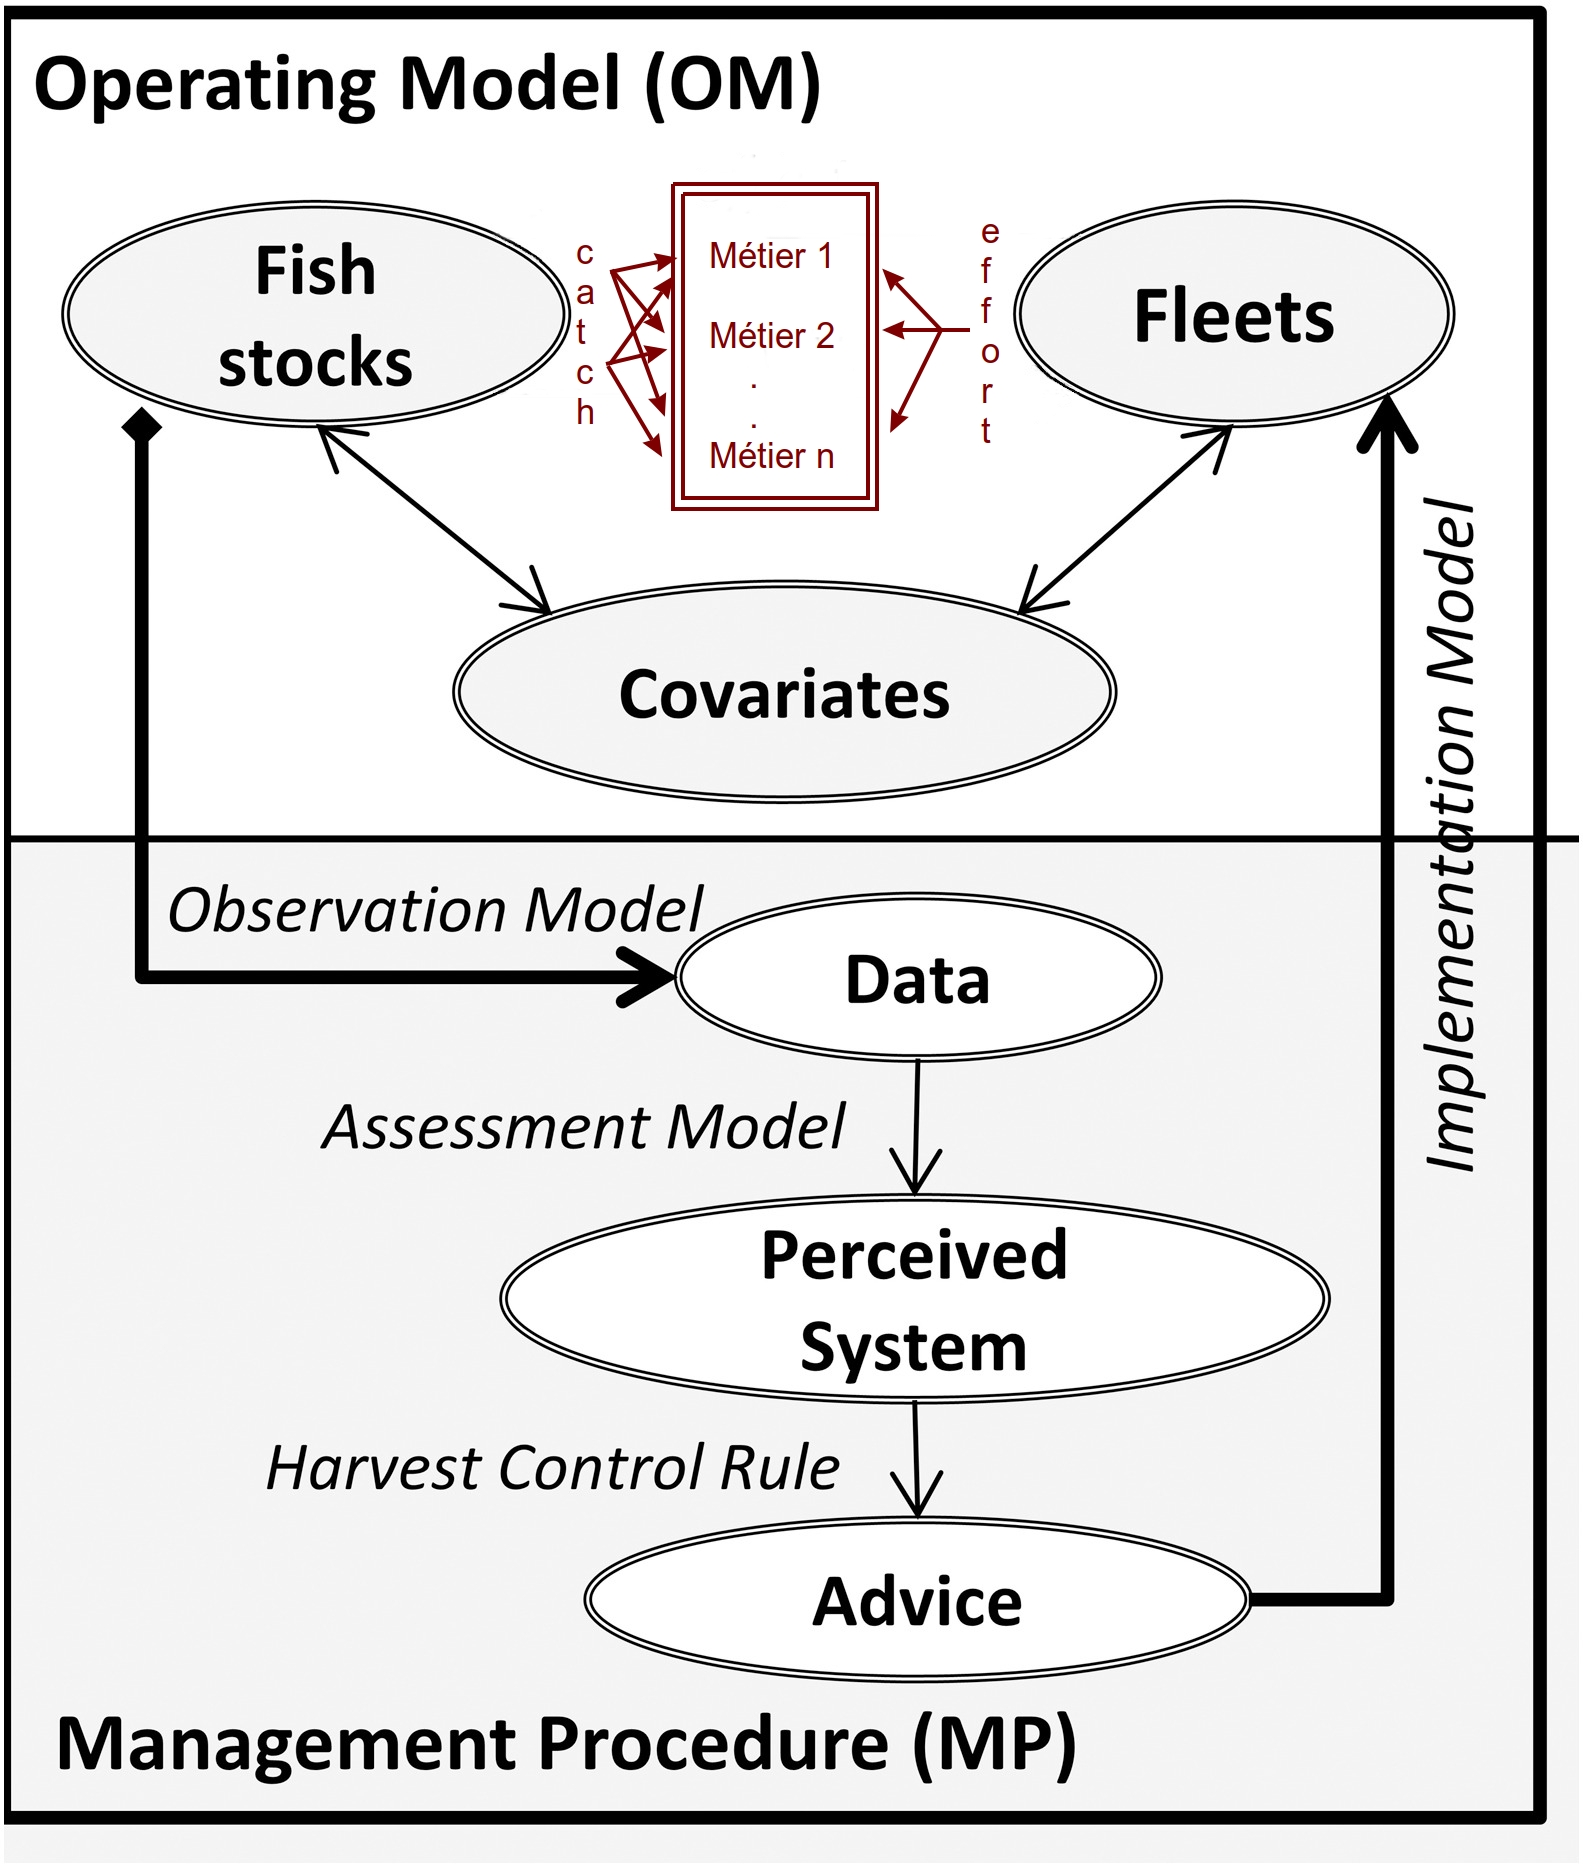
\includegraphics[width=0.6\linewidth]{figures/FLBEIA}
	\caption{FLBEIA schematic, adapted from \cite{Garcia2017} to show the
		métier interaction (dark red) in the modelling framework.} 
	\label{fig:flbeia}
\end{figure}	


\begin{figure}[!ht]
	\centering
\begin{subfigure}
	\centering
	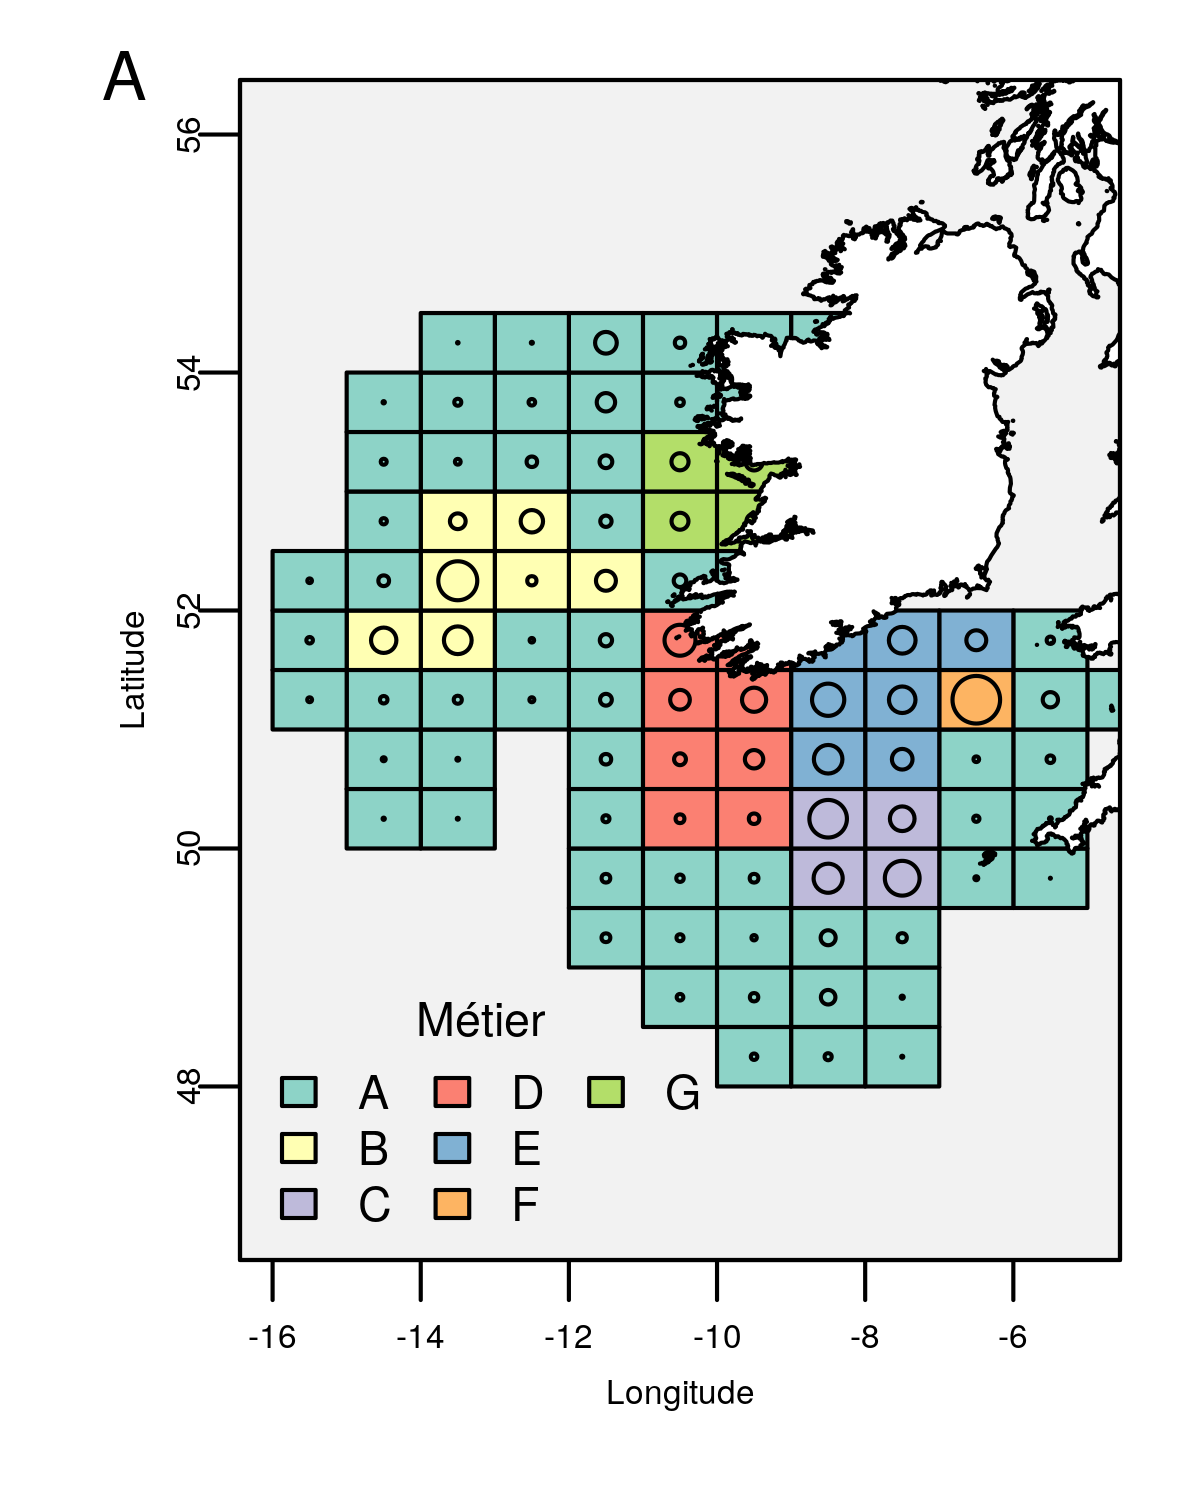
\includegraphics[width=0.6\linewidth]{figures/Final_Metier_locations}
\end{subfigure}
\begin{subfigure}
	\centering
	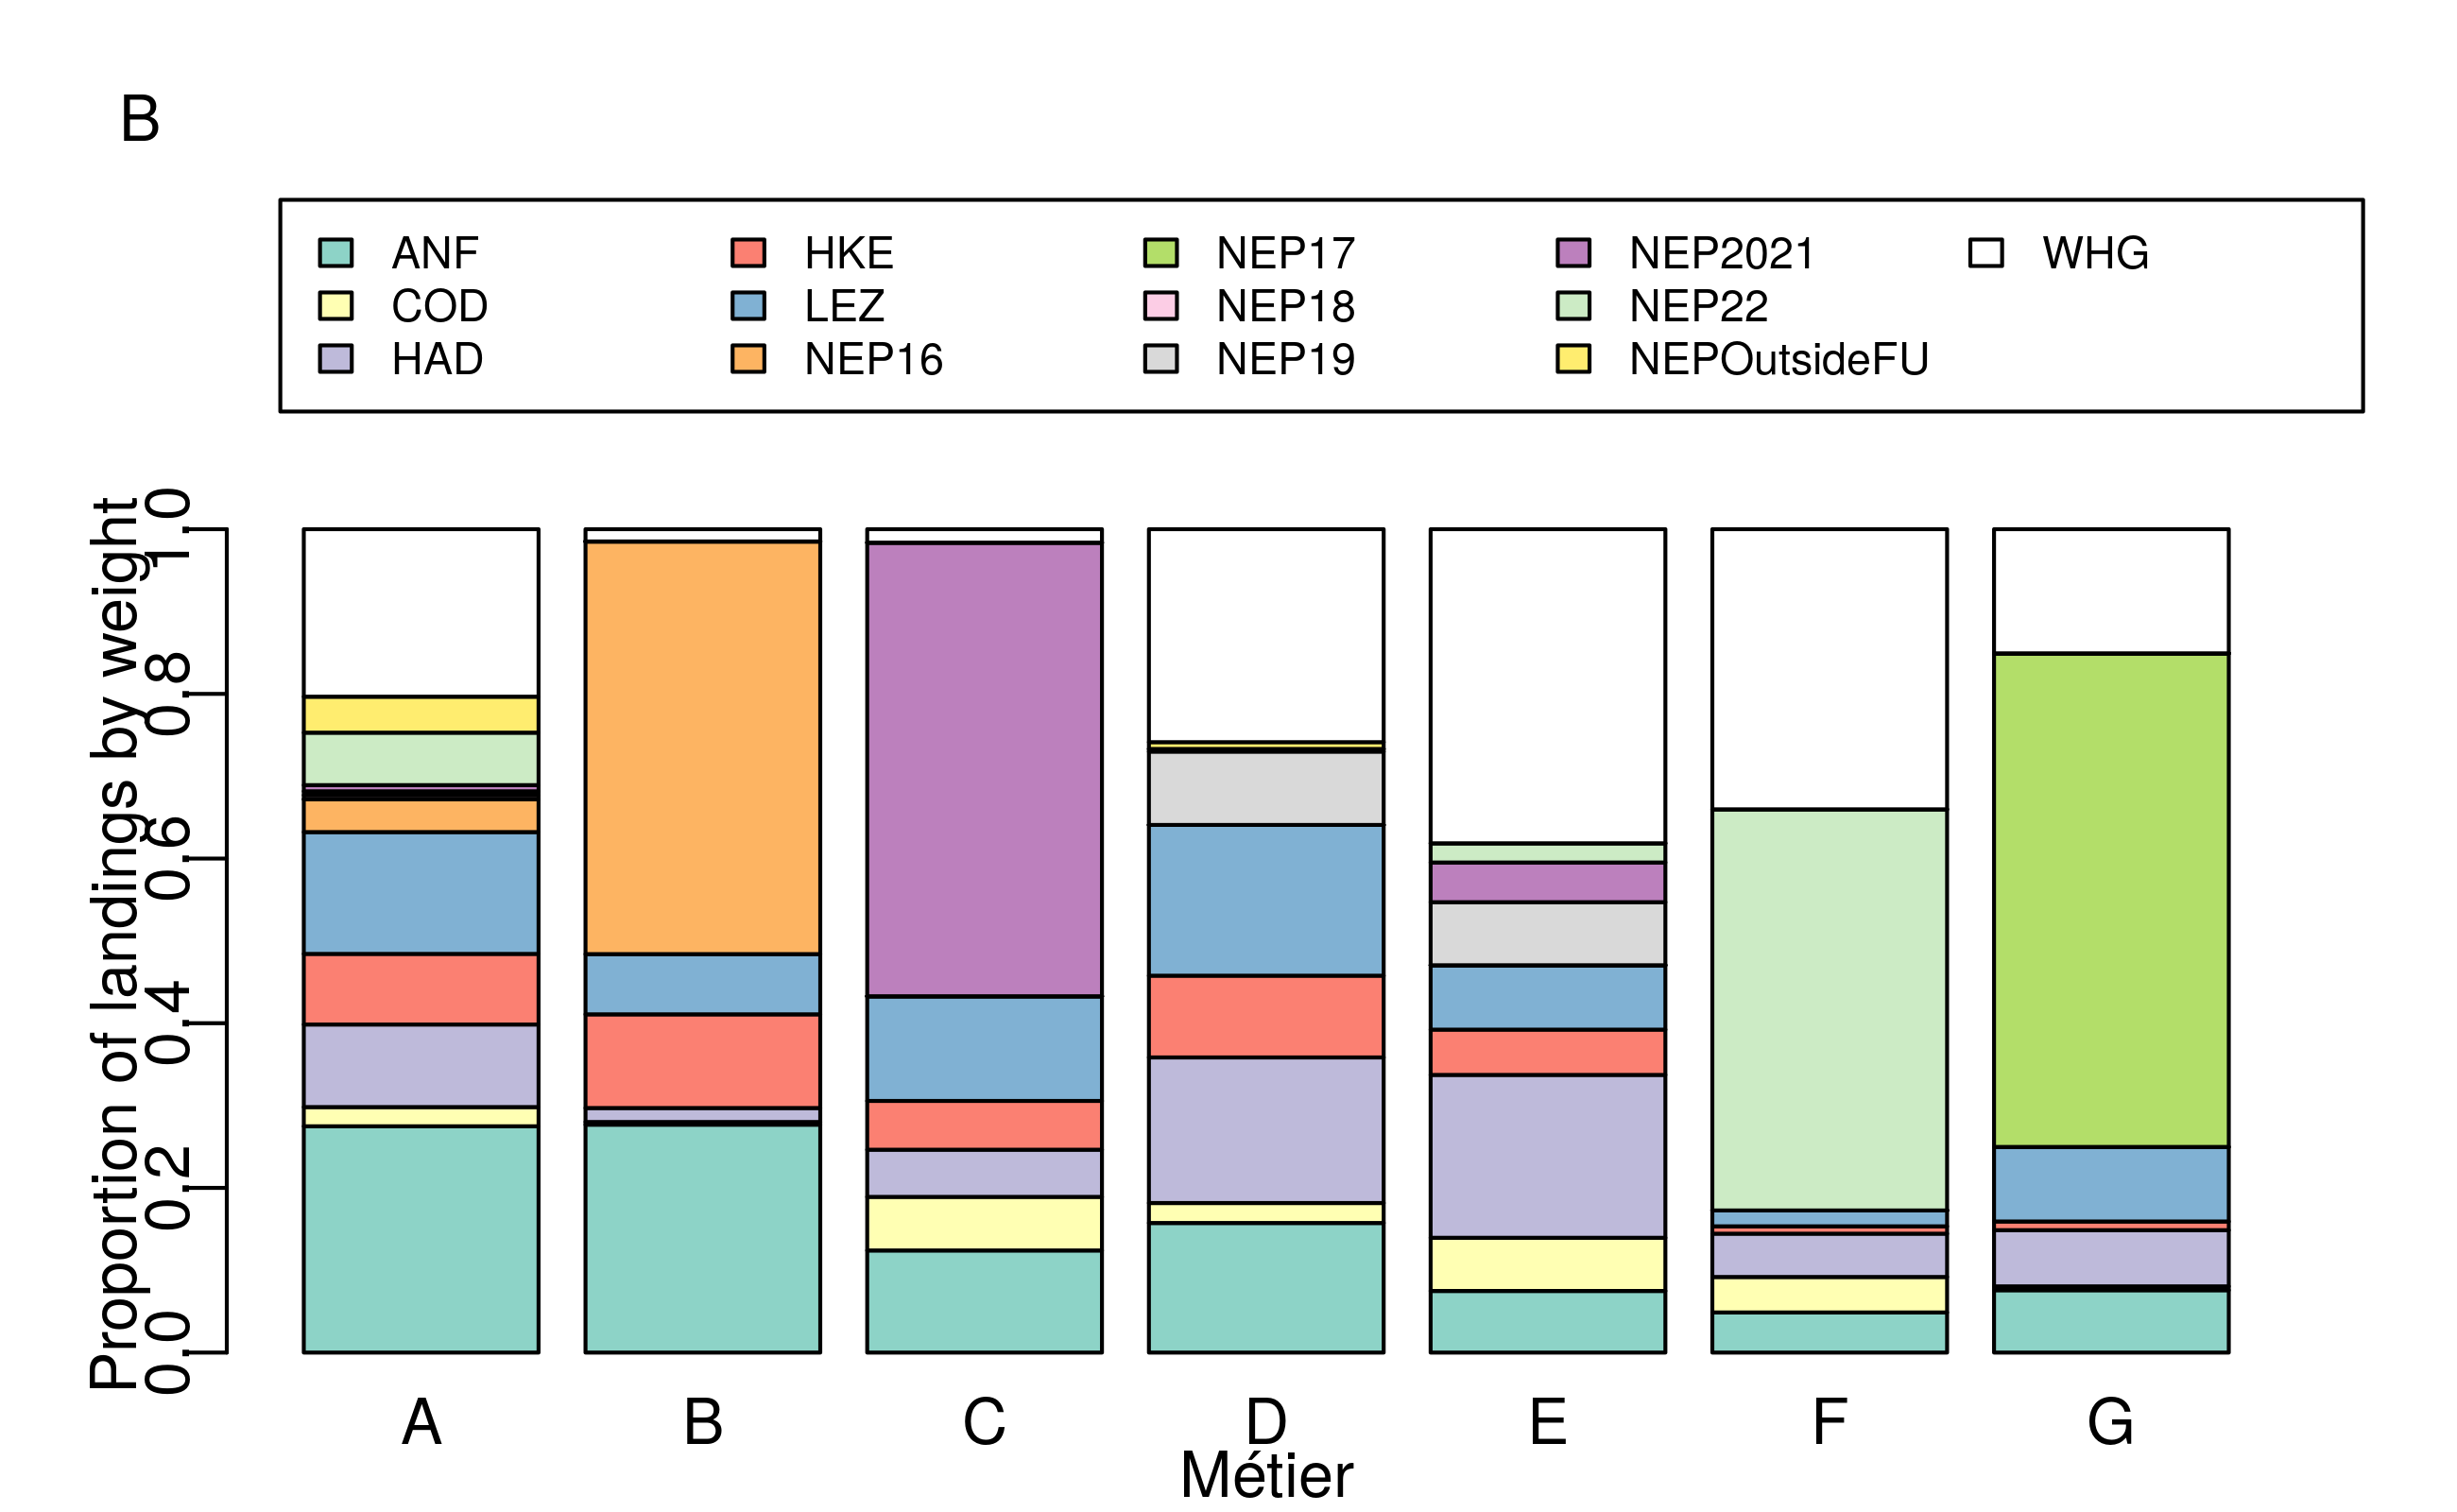
\includegraphics[width=0.8\linewidth]{figures/Final_Metier_catchcomp}
\end{subfigure}
\caption{The métier defined through spatial clustering of similar catch
	composition for Irish Otter trawlers modified by using knowledge of
	fishing grounds to make coherent spatial units. The circles represent
	relative fishing effort in each of the rectangles. Catch compositions
	for the métier indicating the dominant stocks in catches for each of
	the fishing grounds. Stock codes in Table \ref{tab:brp}.} 
	\label{fig:metier}

\end{figure}	

\newpage

\begin{sidewaysfigure}[!ht]
	\centering
	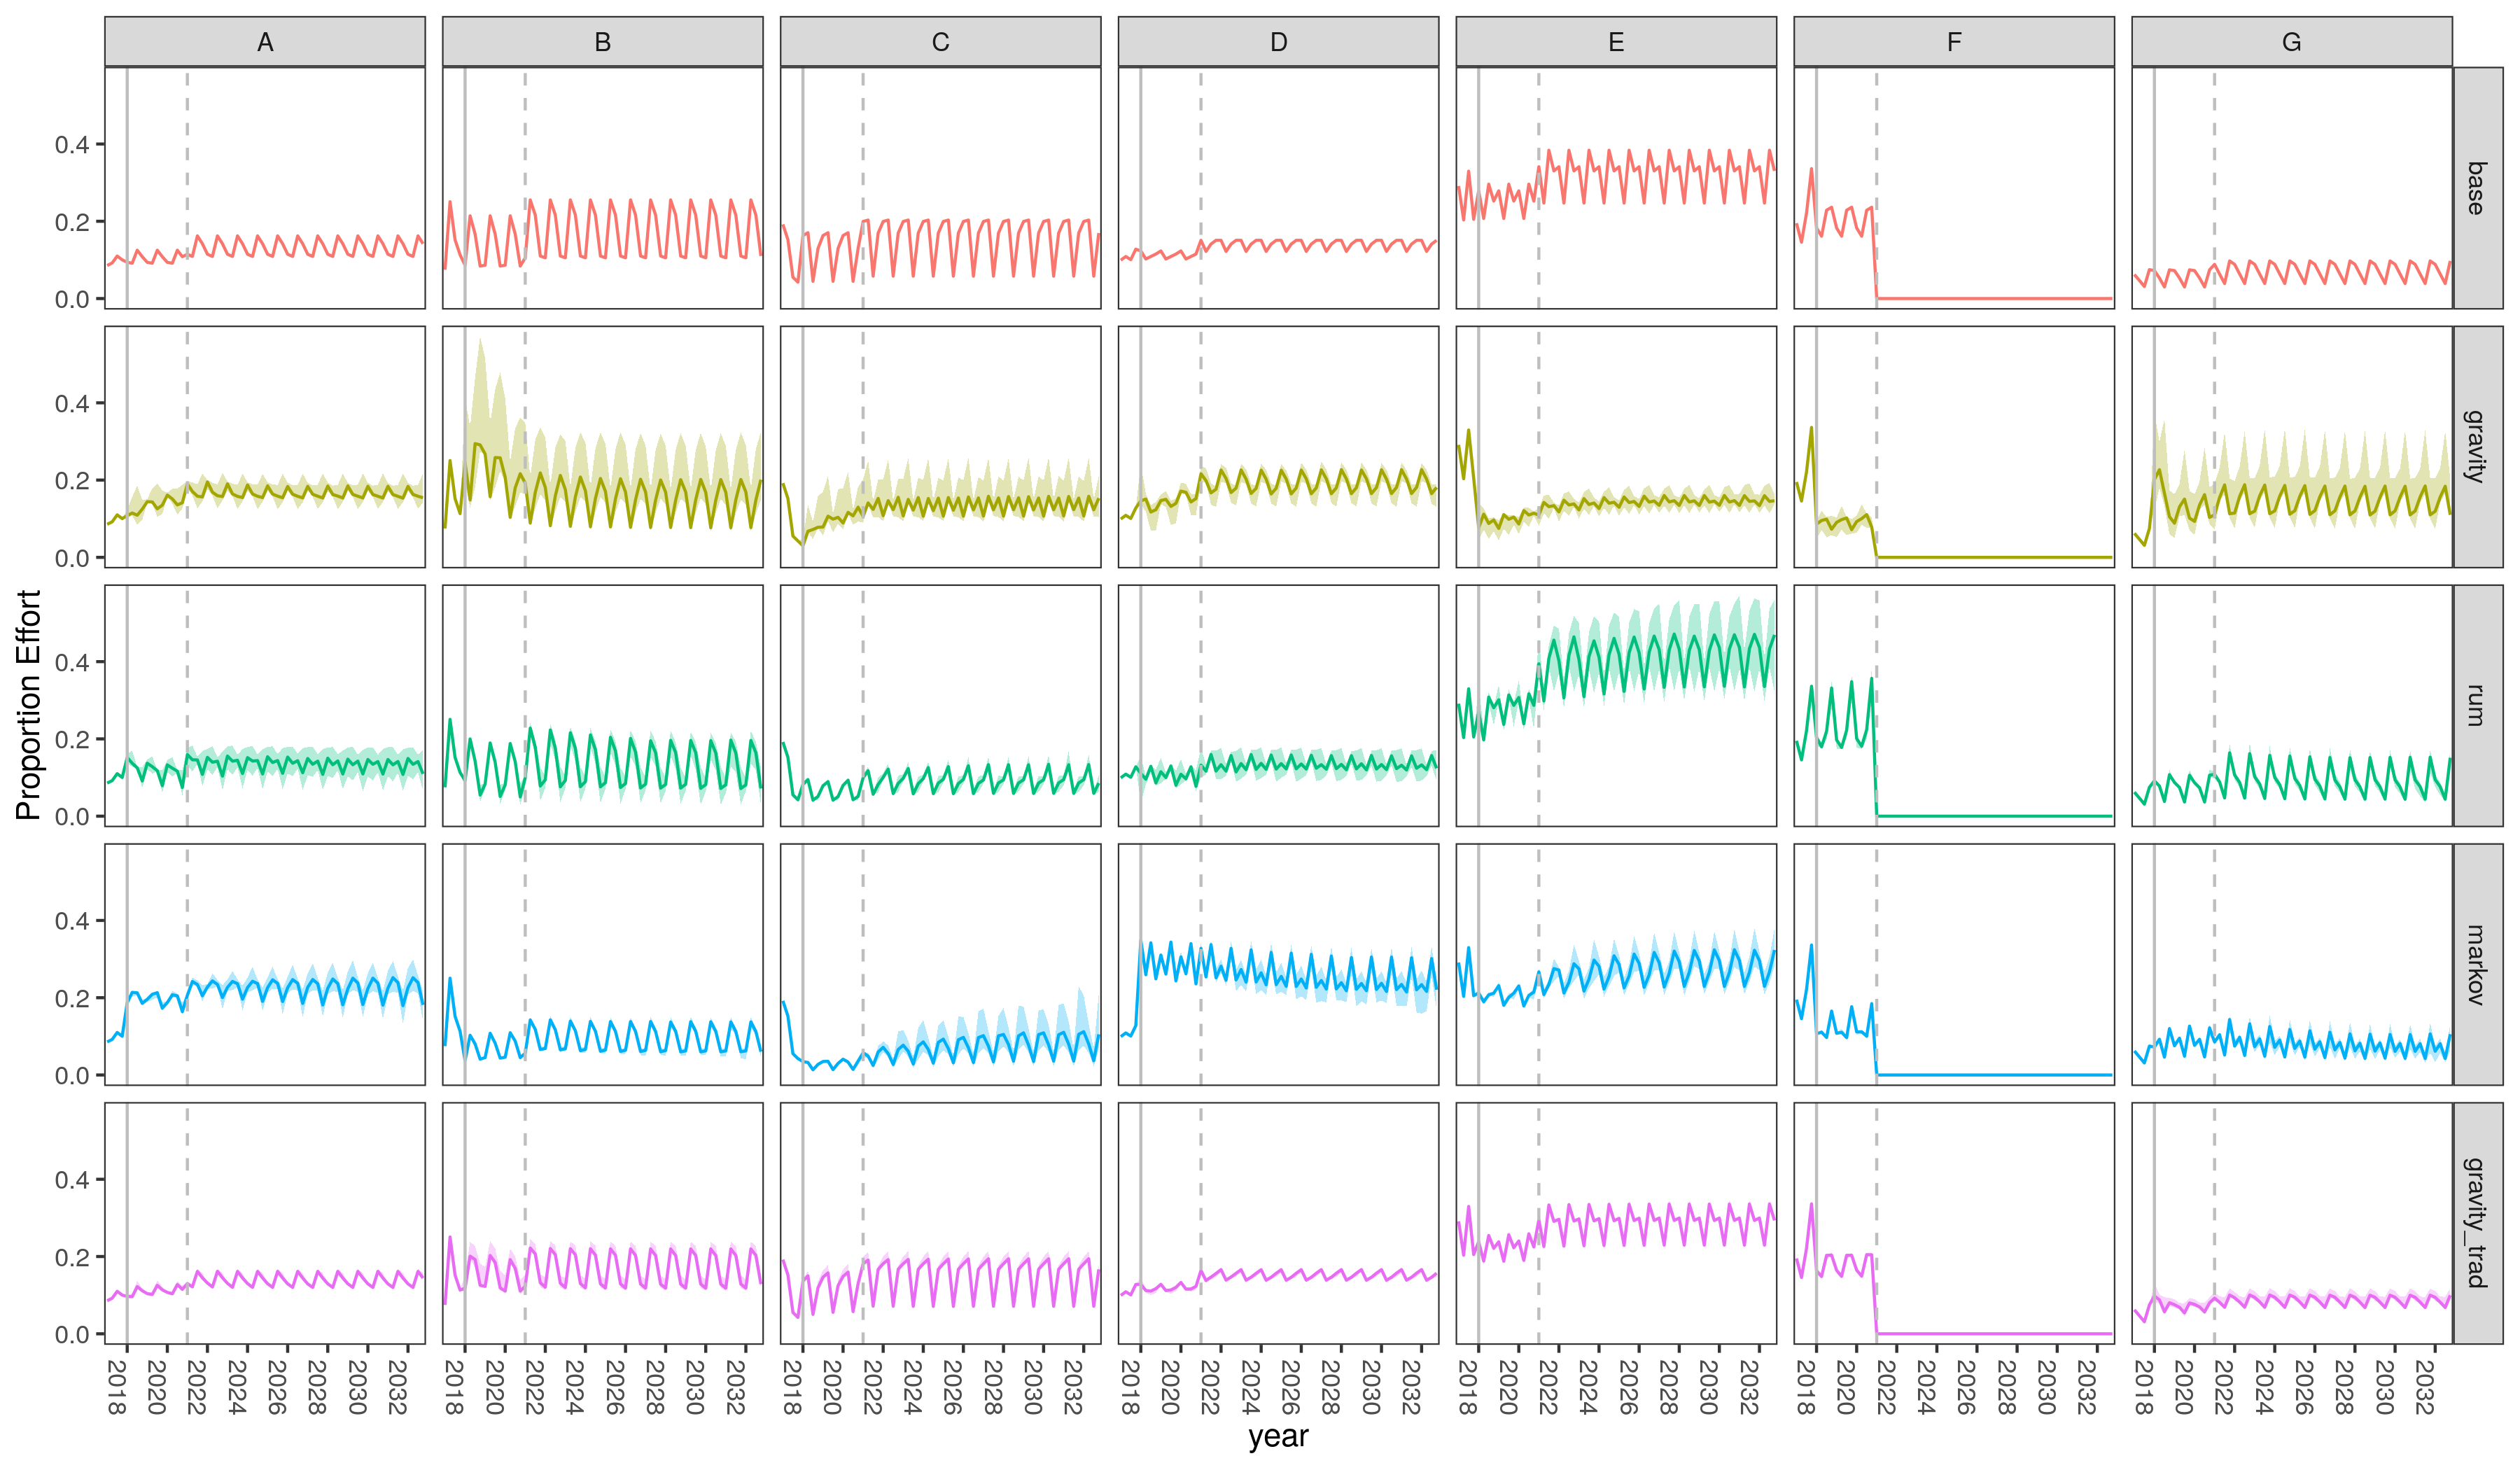
\includegraphics[width=1\linewidth]{figures/Effort_shares}
	\caption{Quarterly fishing effort share (proportion) for each métier
		and location choice model (2017 - 2032). Light shading
		represents 5\% and 95\% variability due to recruitment and
		catchability. Solid line indicates end of the data/start of
		simulations and the dashed line the implementation of the
		spatial closure.} 
	\label{fig:effort}
\end{sidewaysfigure}	

\newpage

\begin{figure}[!ht]
	\centering
	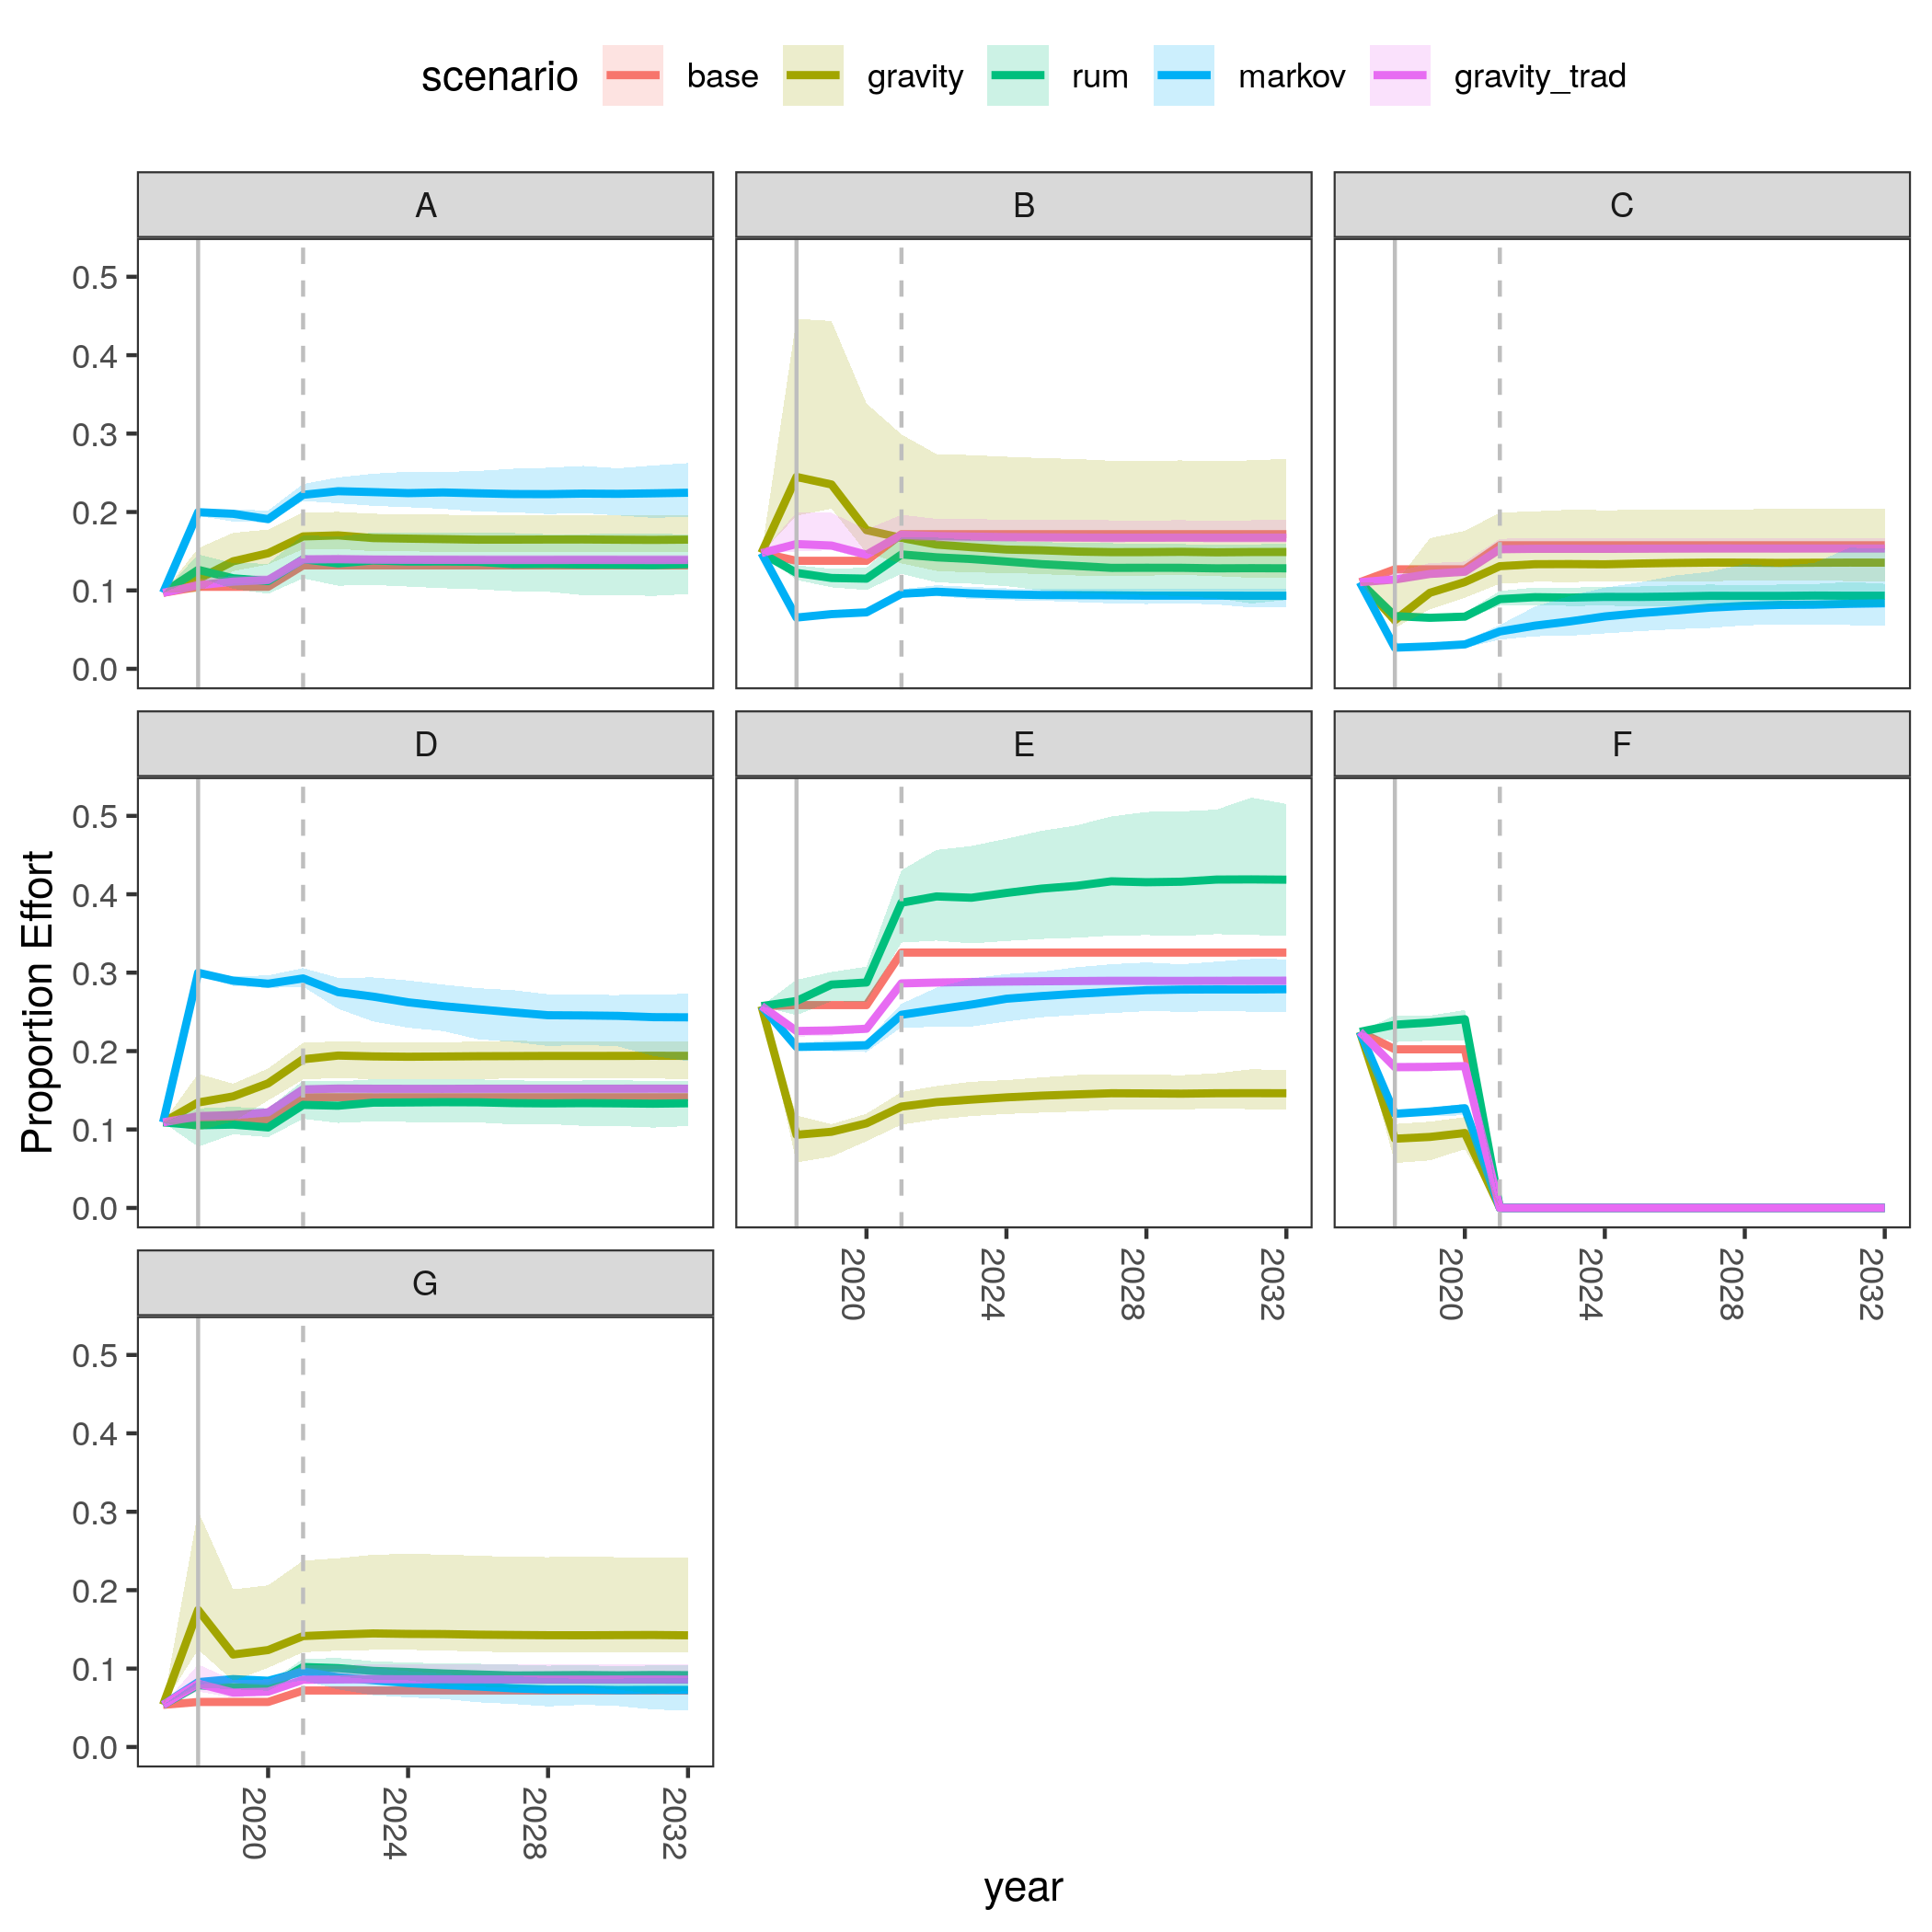
\includegraphics[width=1\linewidth]{figures/Effort_shares_annual}
	\caption{Annualised effort share (proportion) for each métier
		and location choice model (2017 - 2032). Light shading
		represents 5\% and 95\% variability due to recruitment and
		catchability. Solid line indicates end of the data/start of
		simulations and the dashed line the implementation of the
		spatial closure.} 
	\label{fig:effort_an}
\end{figure}	

\begin{figure}[!ht]
	\centering
	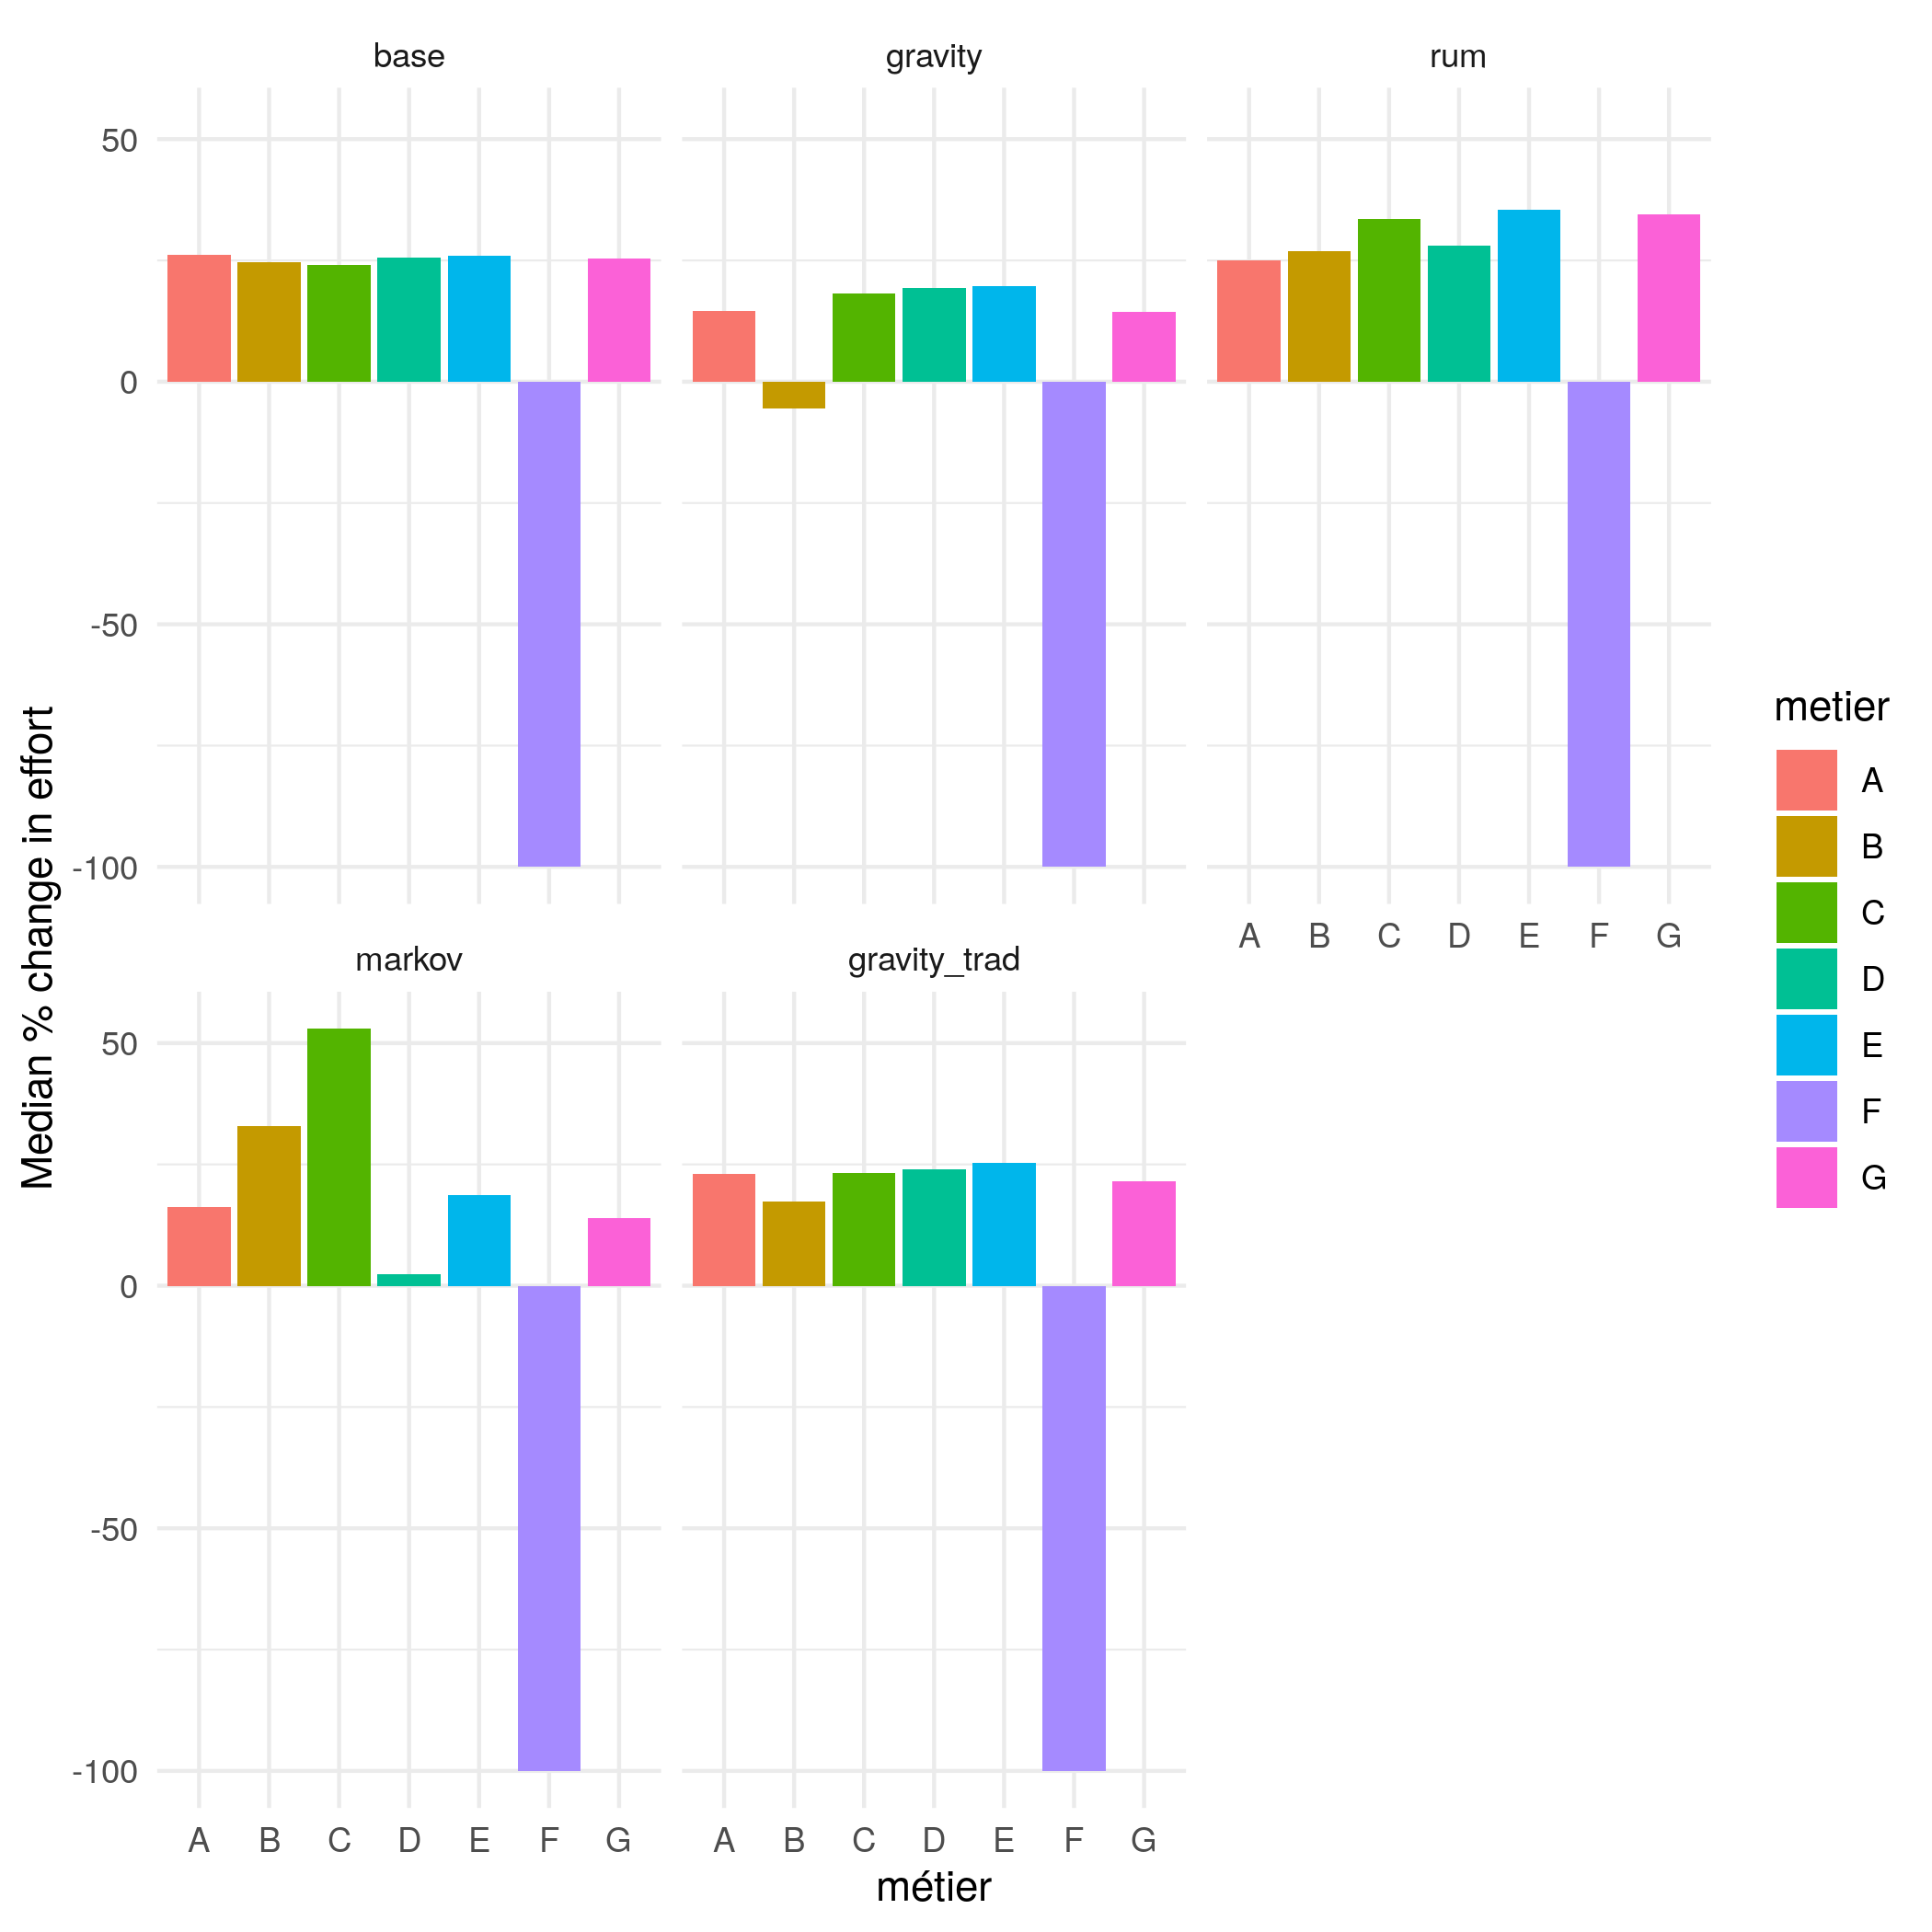
\includegraphics[width=1\linewidth]{figures/Change_effort}
	\caption{Percentage change in annualised effort share for each of the
		métier from before (2020) the closure of métier F and first
		year of the closure (2021).} 
	\label{fig:effort_chg}
\end{figure}	

\begin{figure}[!ht]
	\centering
	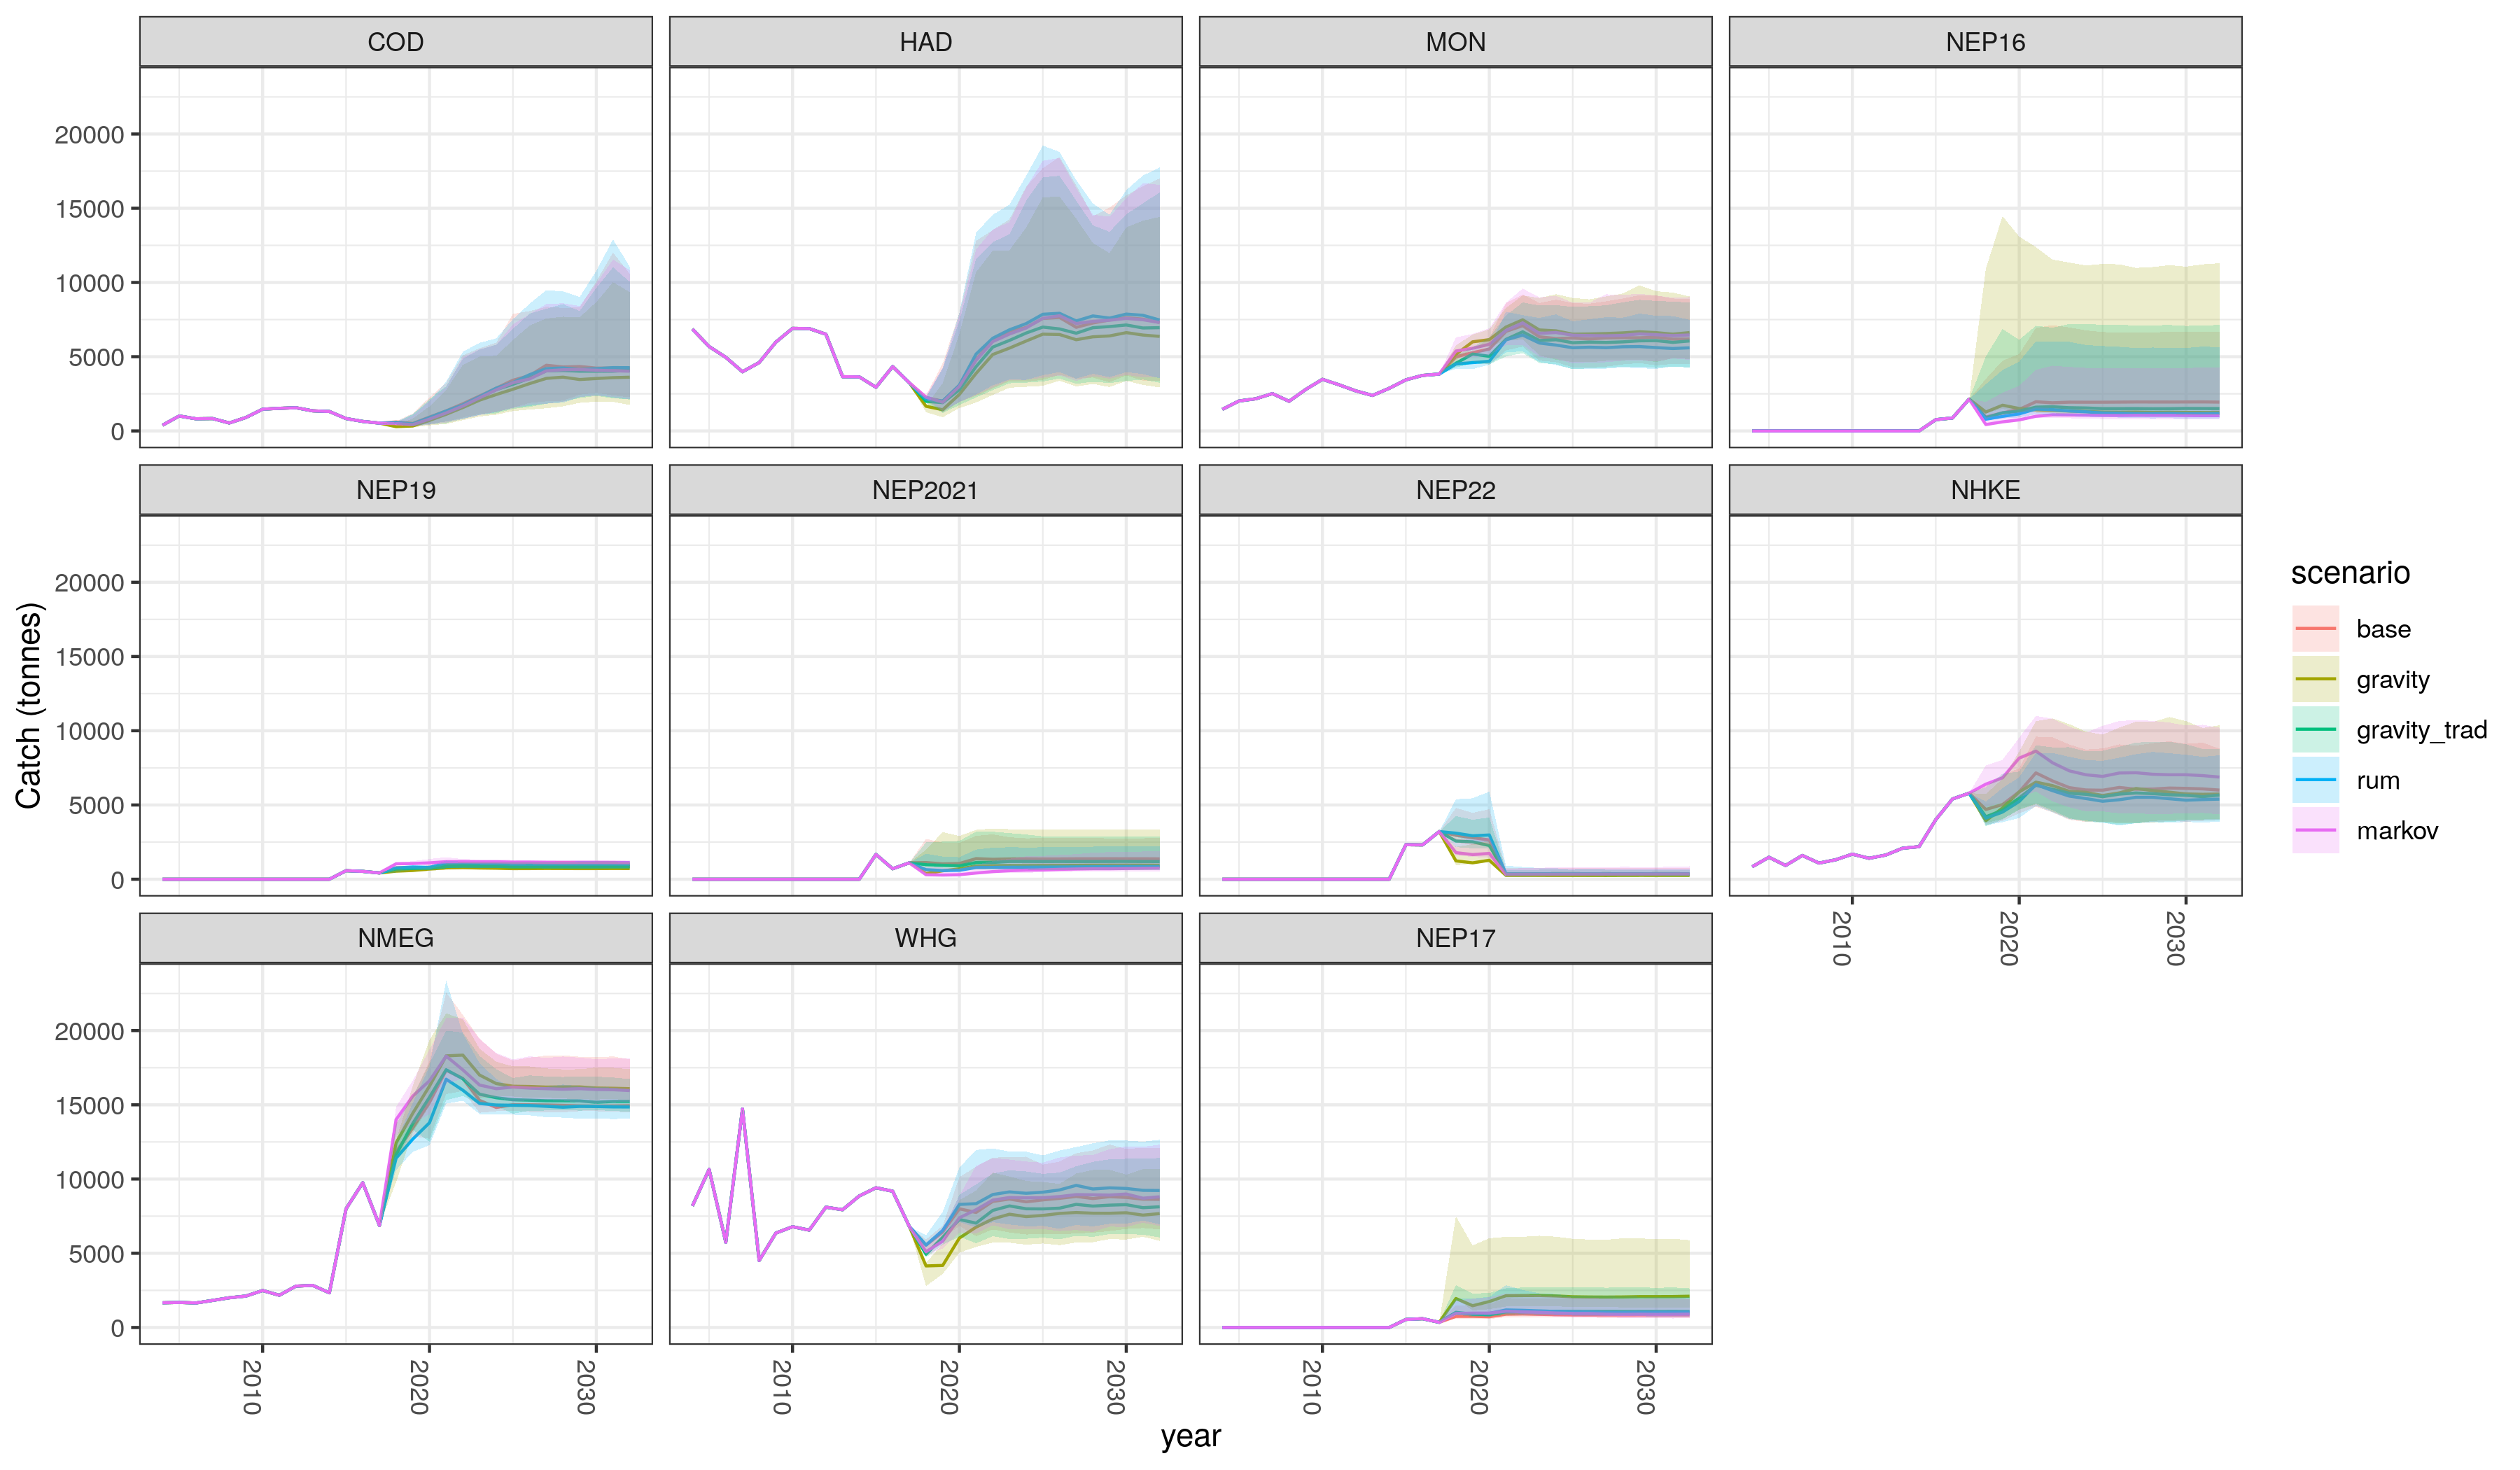
\includegraphics[width=1\linewidth]{figures/IE_Otter_catches}
	\caption{Catches of each stock by Irish Otter trawlers under the
		different location choice models. Light shading represents 5\%
		and 95\% variability due to recruitment and catchability. Solid
		line indicates end of the data/start of simulations and the
		dashed line the implementation of the spatial closure.} 
	\label{fig:OtterC}
\end{figure}	

\begin{figure}[!ht]
	\centering
	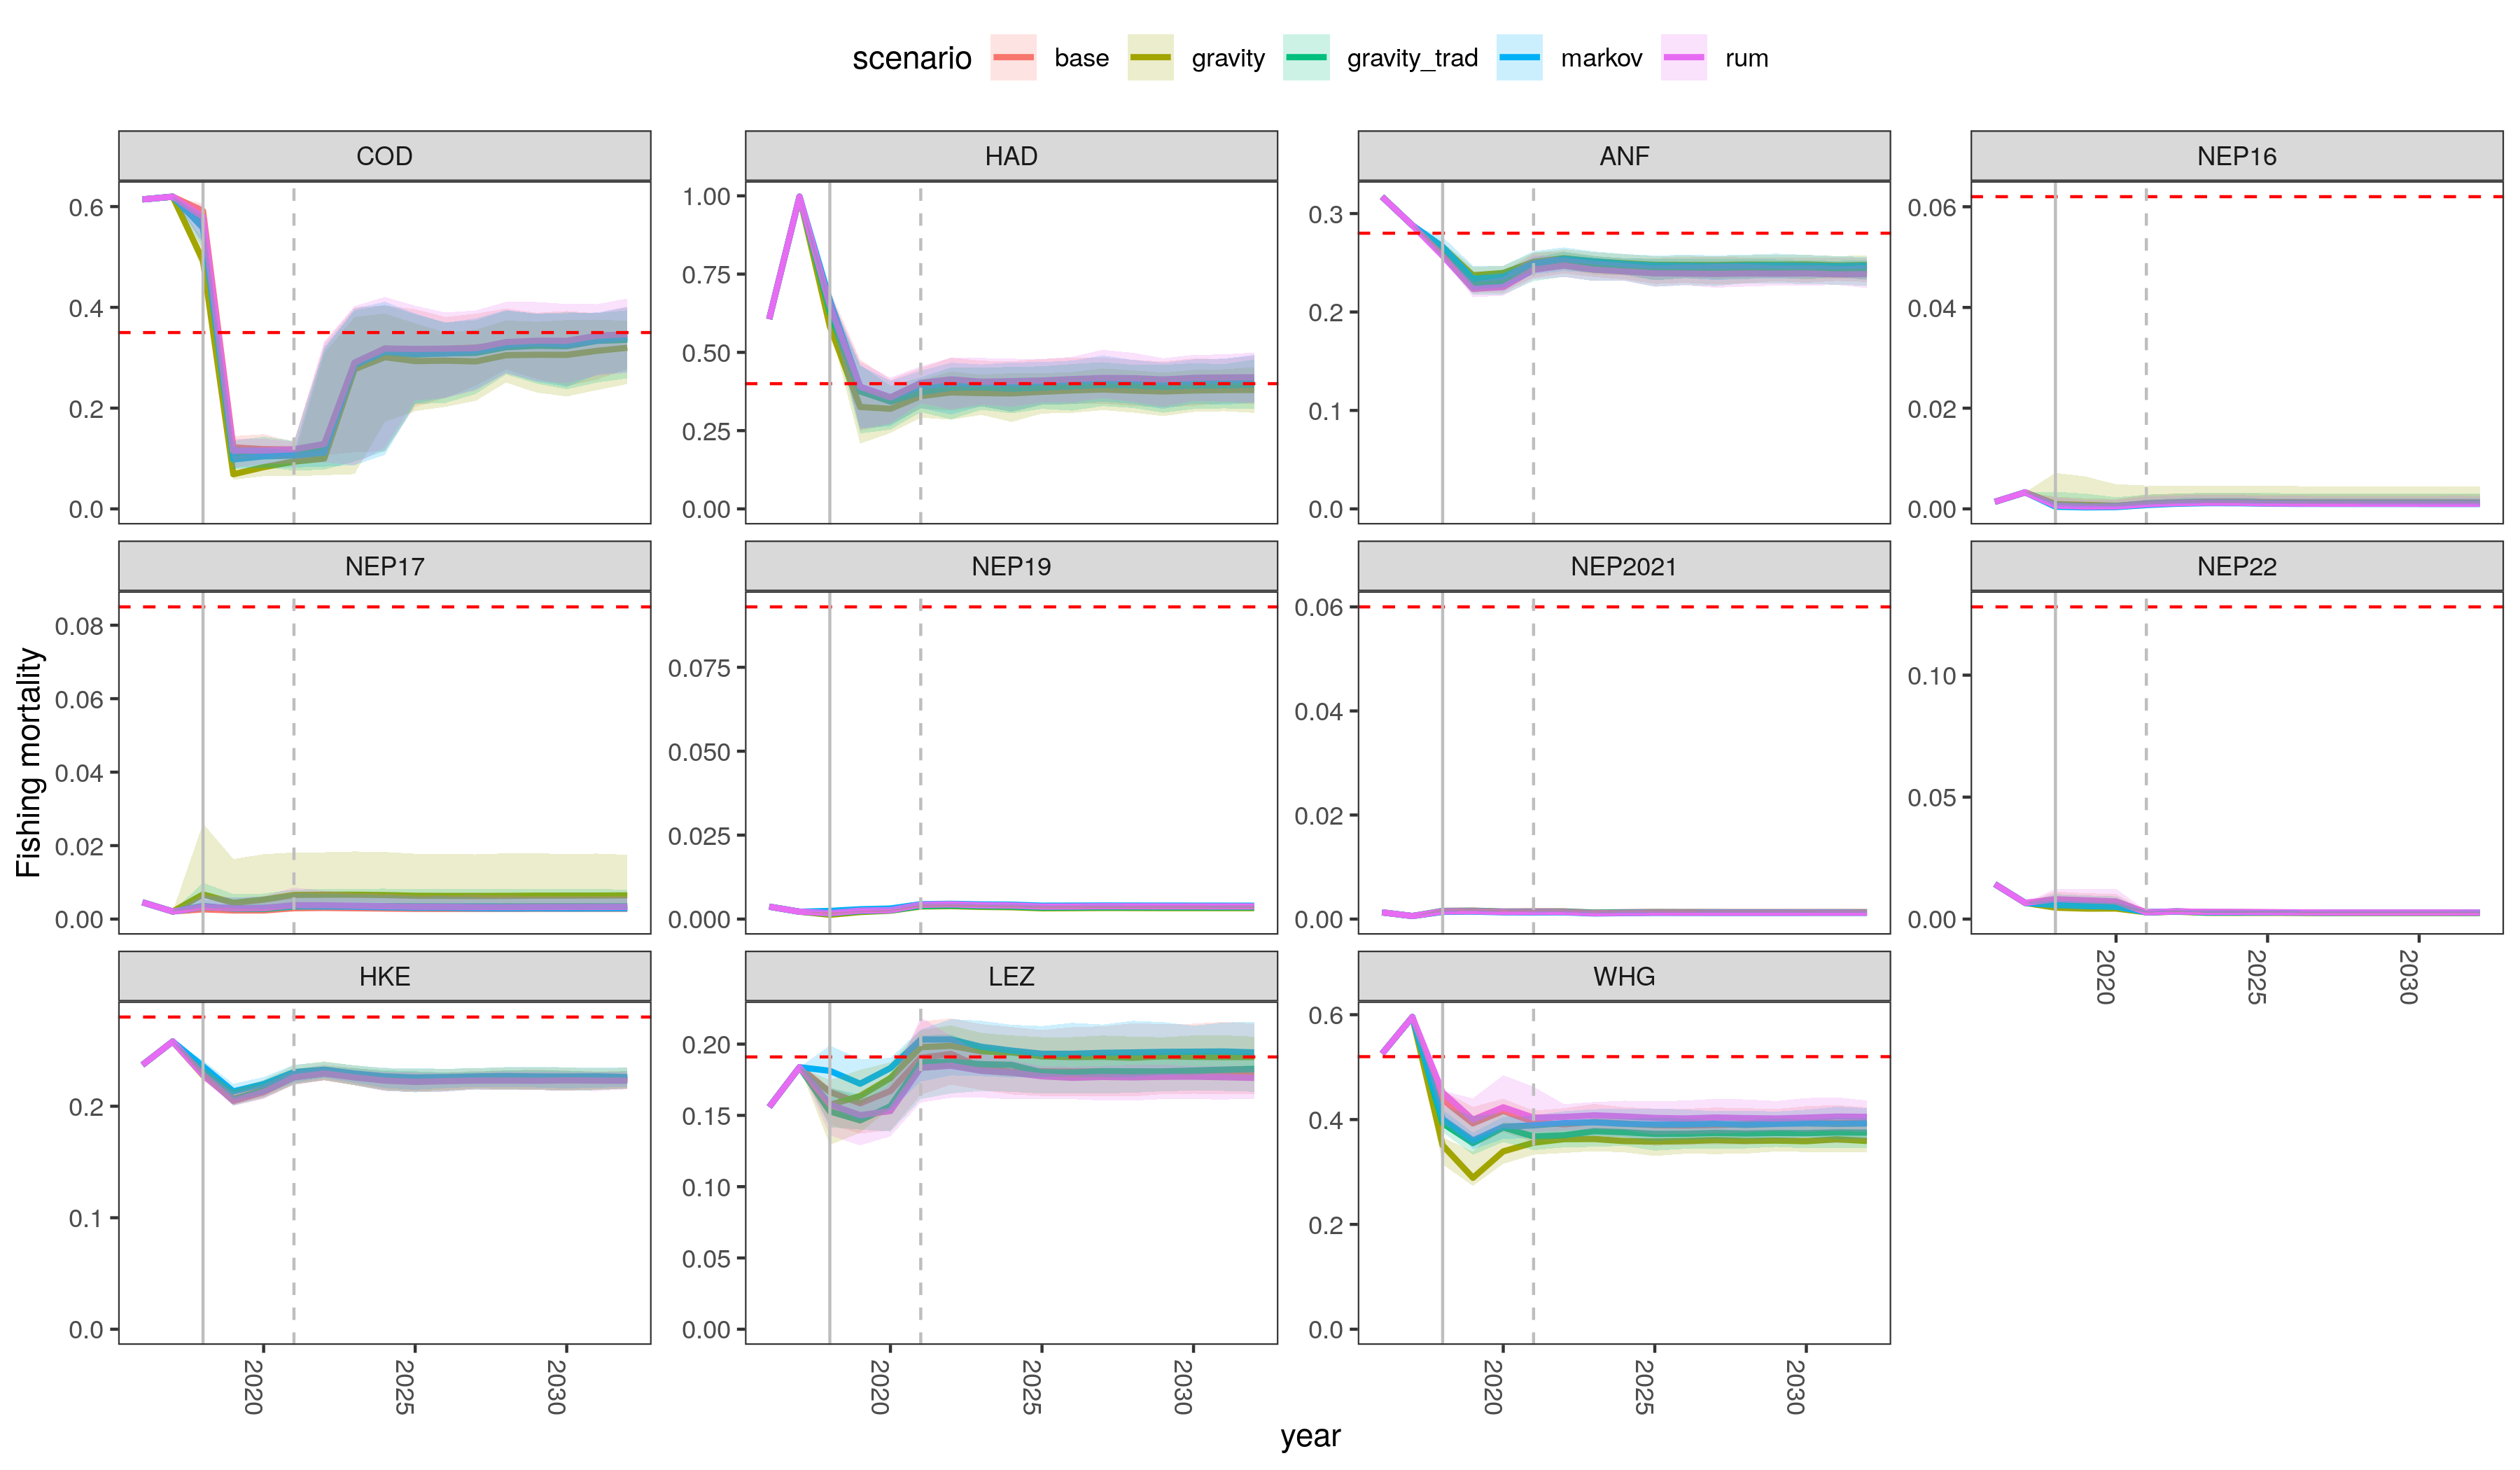
\includegraphics[width=1\linewidth]{figures/F_difference}
	\caption{Fishing mortality for each stock under the different location
		choice models. Each stock was targeted to be fished at its Fmsy
		rate, using the ICES MSY Harvest Control Rule. Light shading
		represents 5\% and 95\% variability due to recruitment and
		catchability. Solid line indicates end of the data/start of
		simulations and the dashed line the implementation of the
		spatial closure. Dashed red lines indicate the stock Fmsy
		reference point.} 
	\label{fig:F}
\end{figure}	

\begin{figure}[!ht]
	\centering
	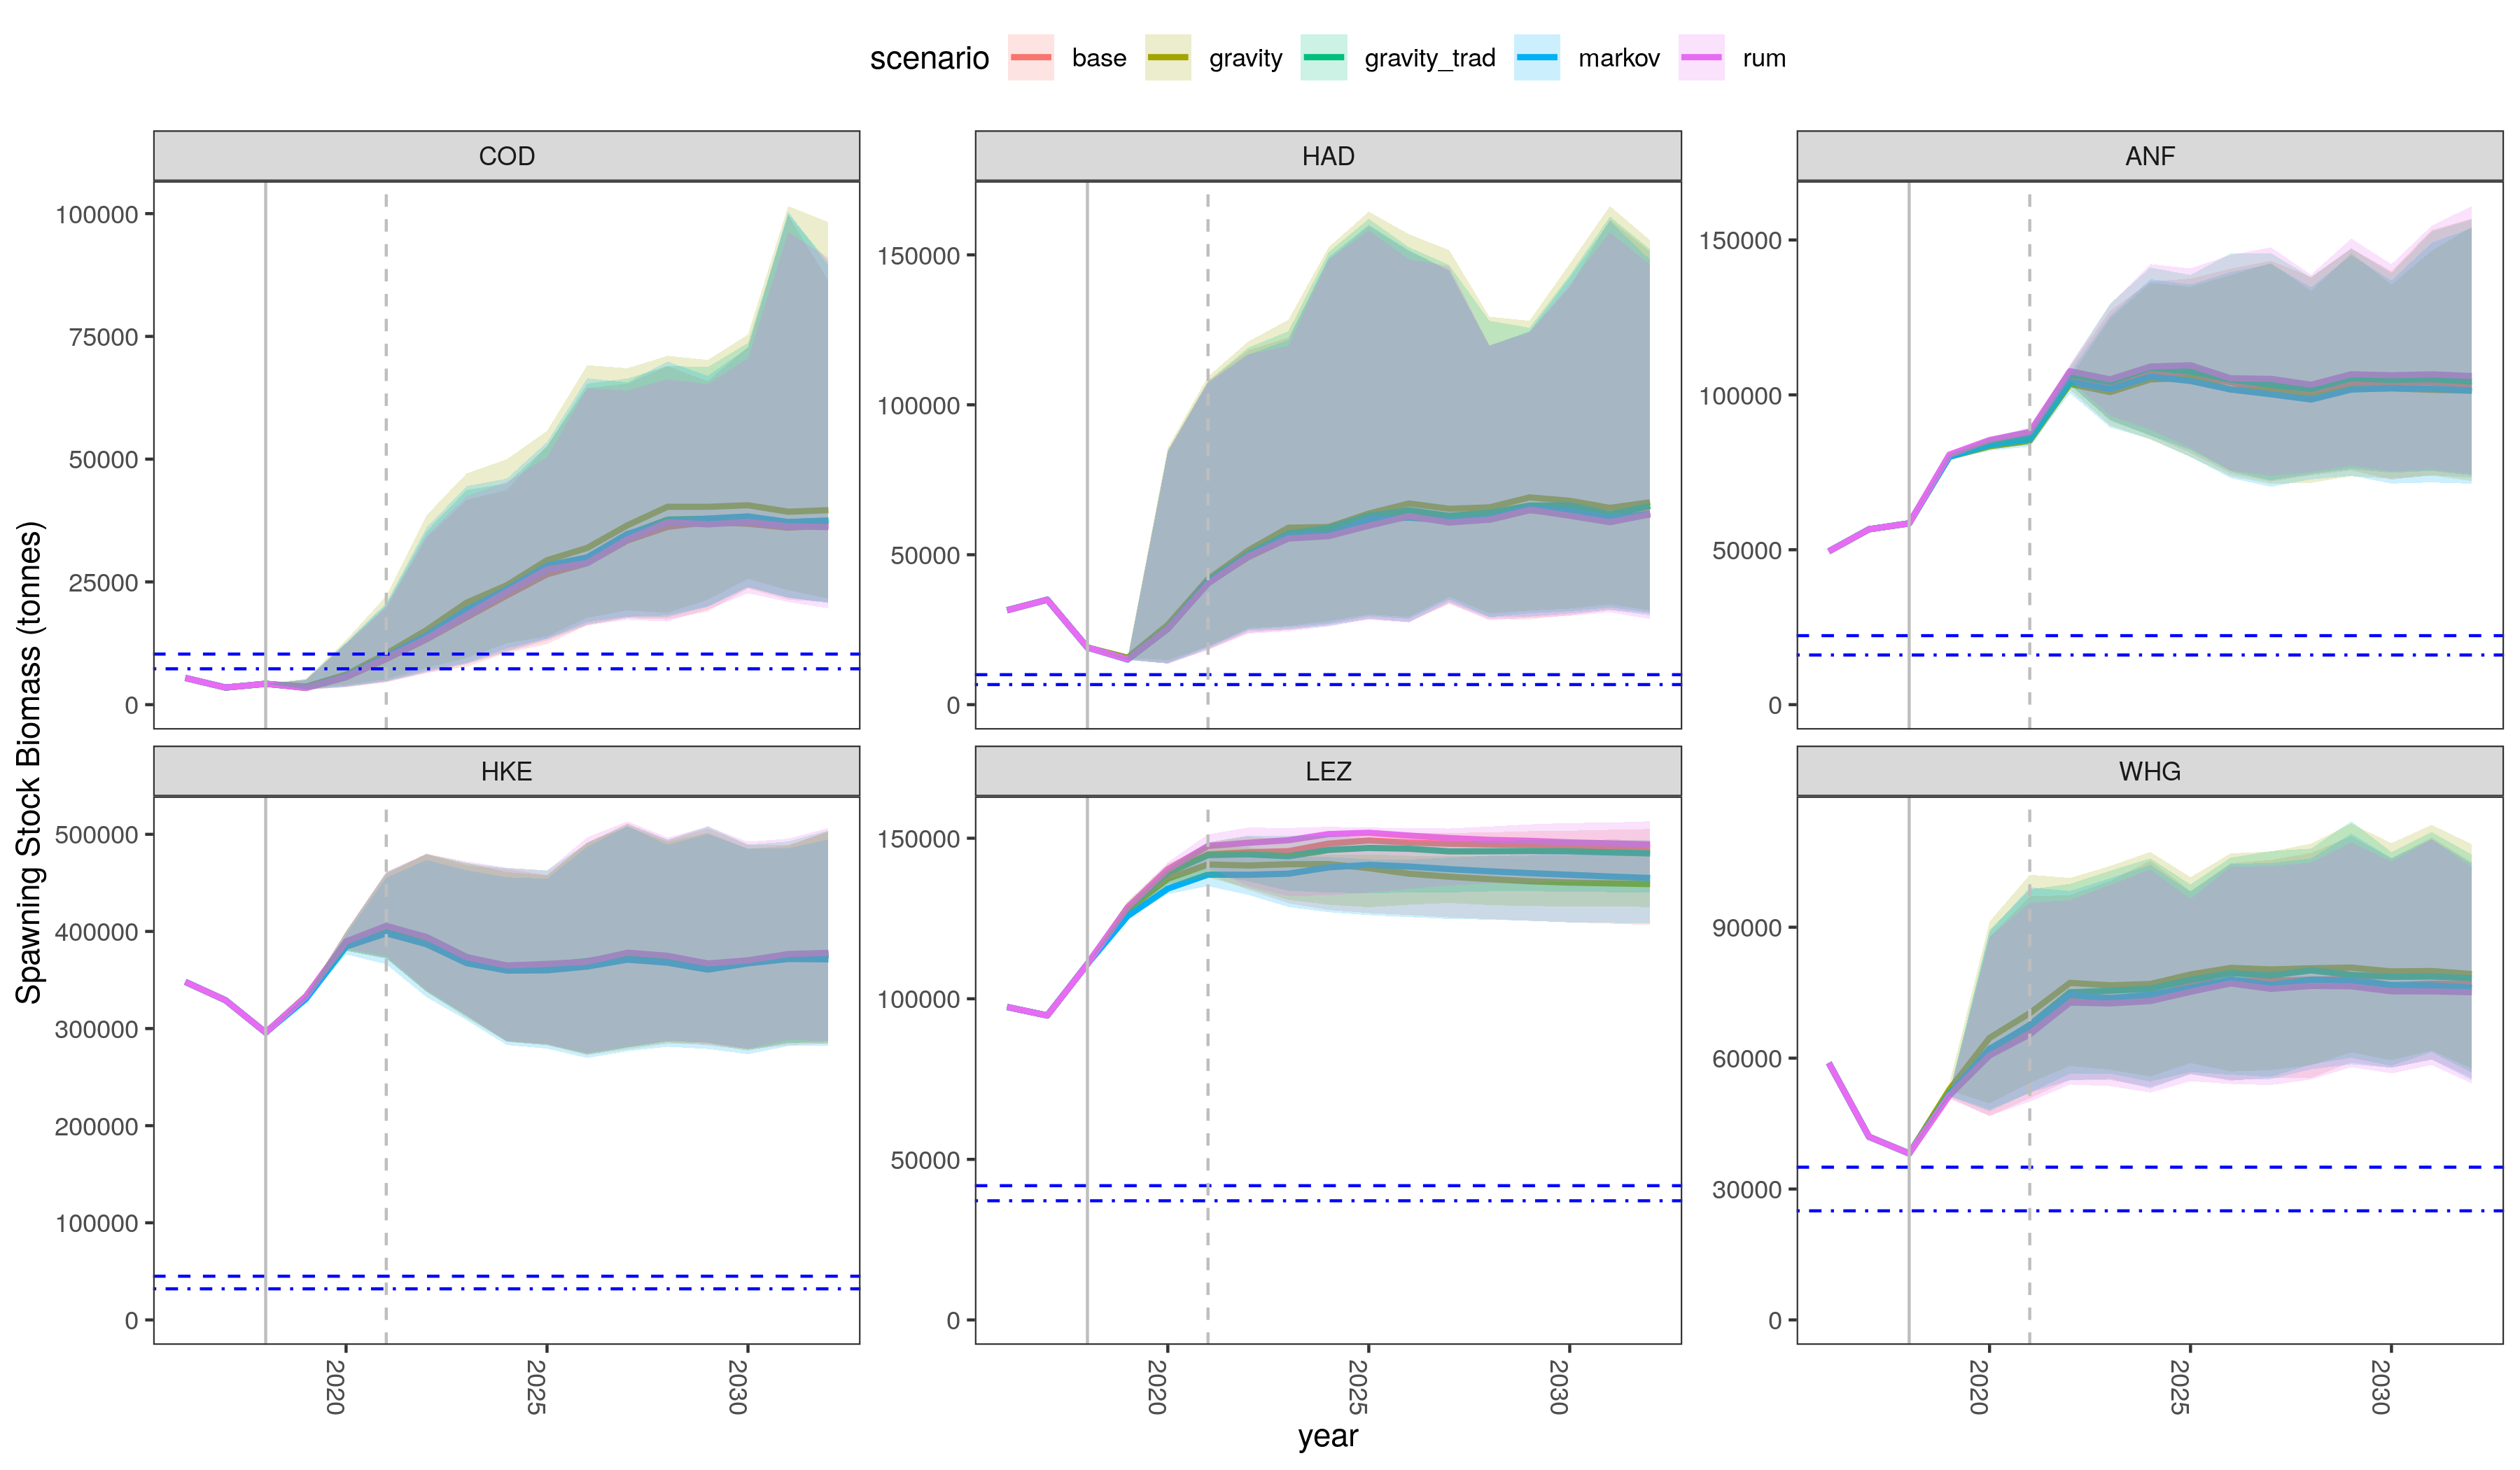
\includegraphics[width=1\linewidth]{figures/SSB_difference}
	\caption{Spawning Stock Biomass for the fish stocks under each location
		model scenario. Light shading represents 5\% and 95\%
		variability due to recruitment and catchability. Solid line
		indicates end of the data/start of simulations and the dashed
		line the implementation of the spatial closure.  Dotdashed and
		dashed blue lines indicate the Blim reference and Bmsytrigger
		reference points respectively.} 
	\label{fig:SSB}
\end{figure}	

\begin{figure}[!ht]
	\centering
	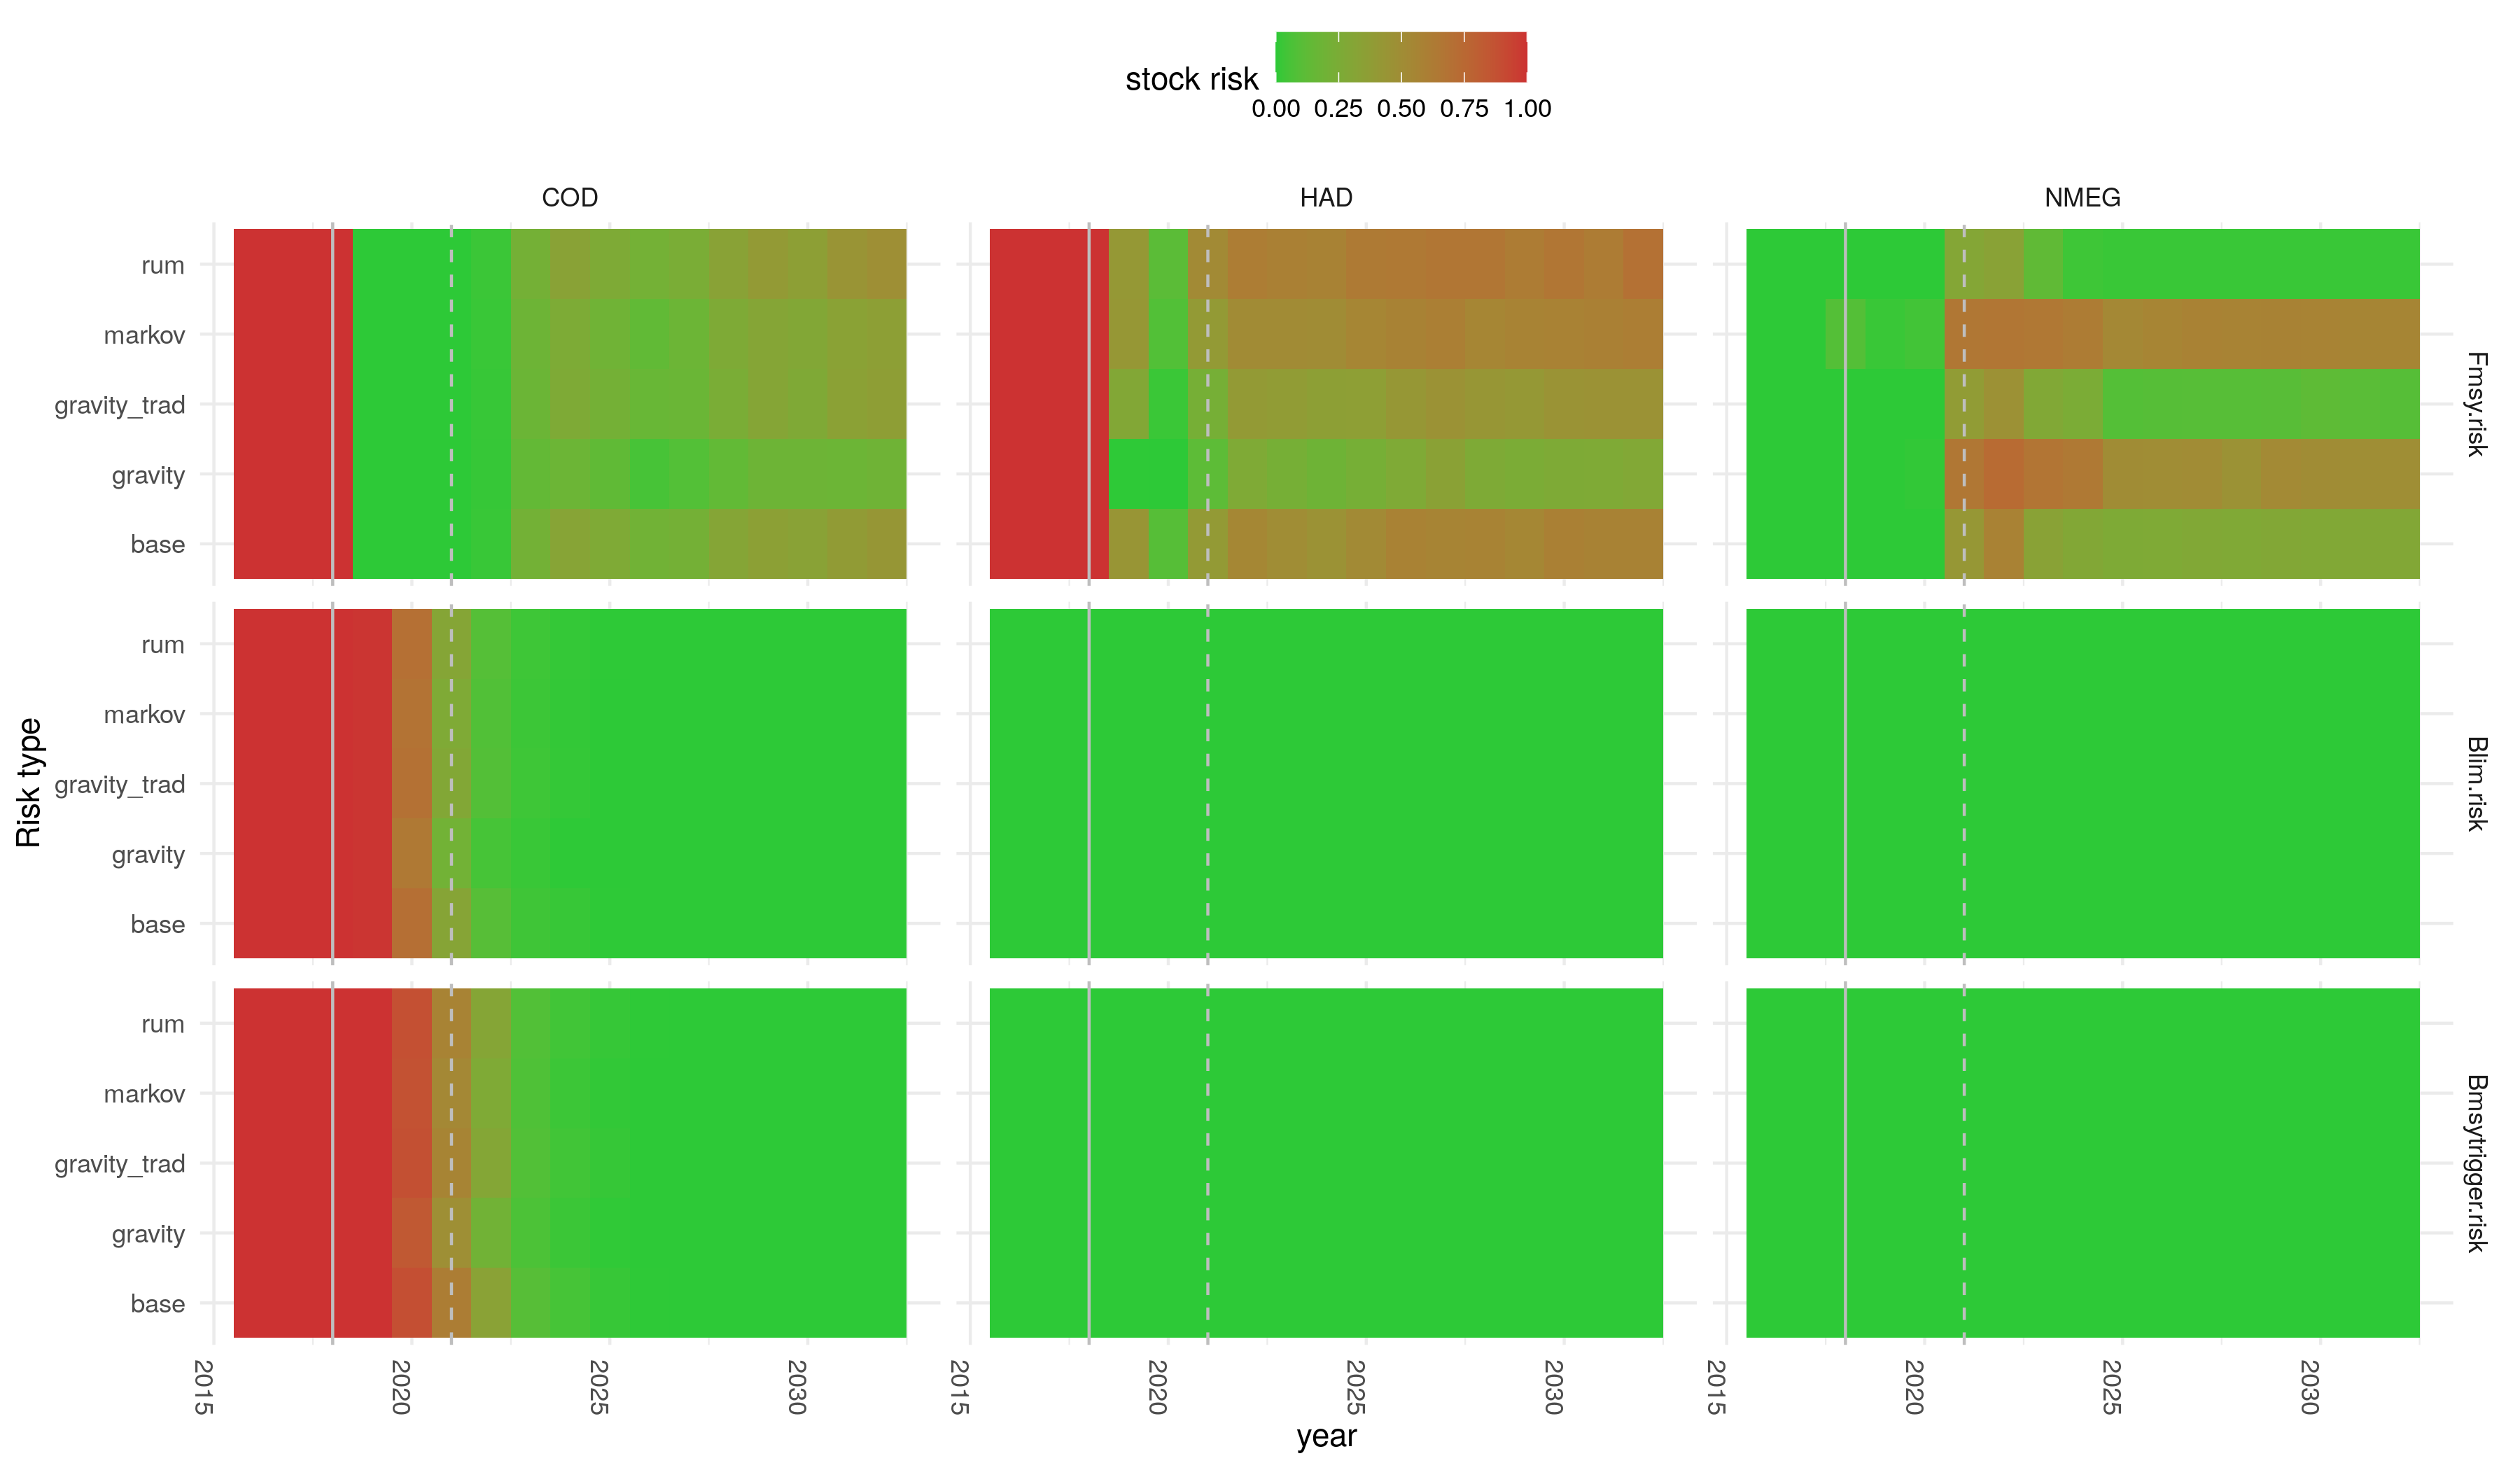
\includegraphics[width=1\linewidth]{figures/stock_risks}
	\caption{Stock risk indicators for each of the fish stock and location
		choice model scenarios. Solid
		line indicates end of the data/start of simulations and the
		dashed line the implementation of the spatial closure.} 
	\label{fig:risk}
\end{figure}	

\clearpage

\section{Appendices}

\textbf{Appendix A}

\begin{figure}[!ht]
	\centering
	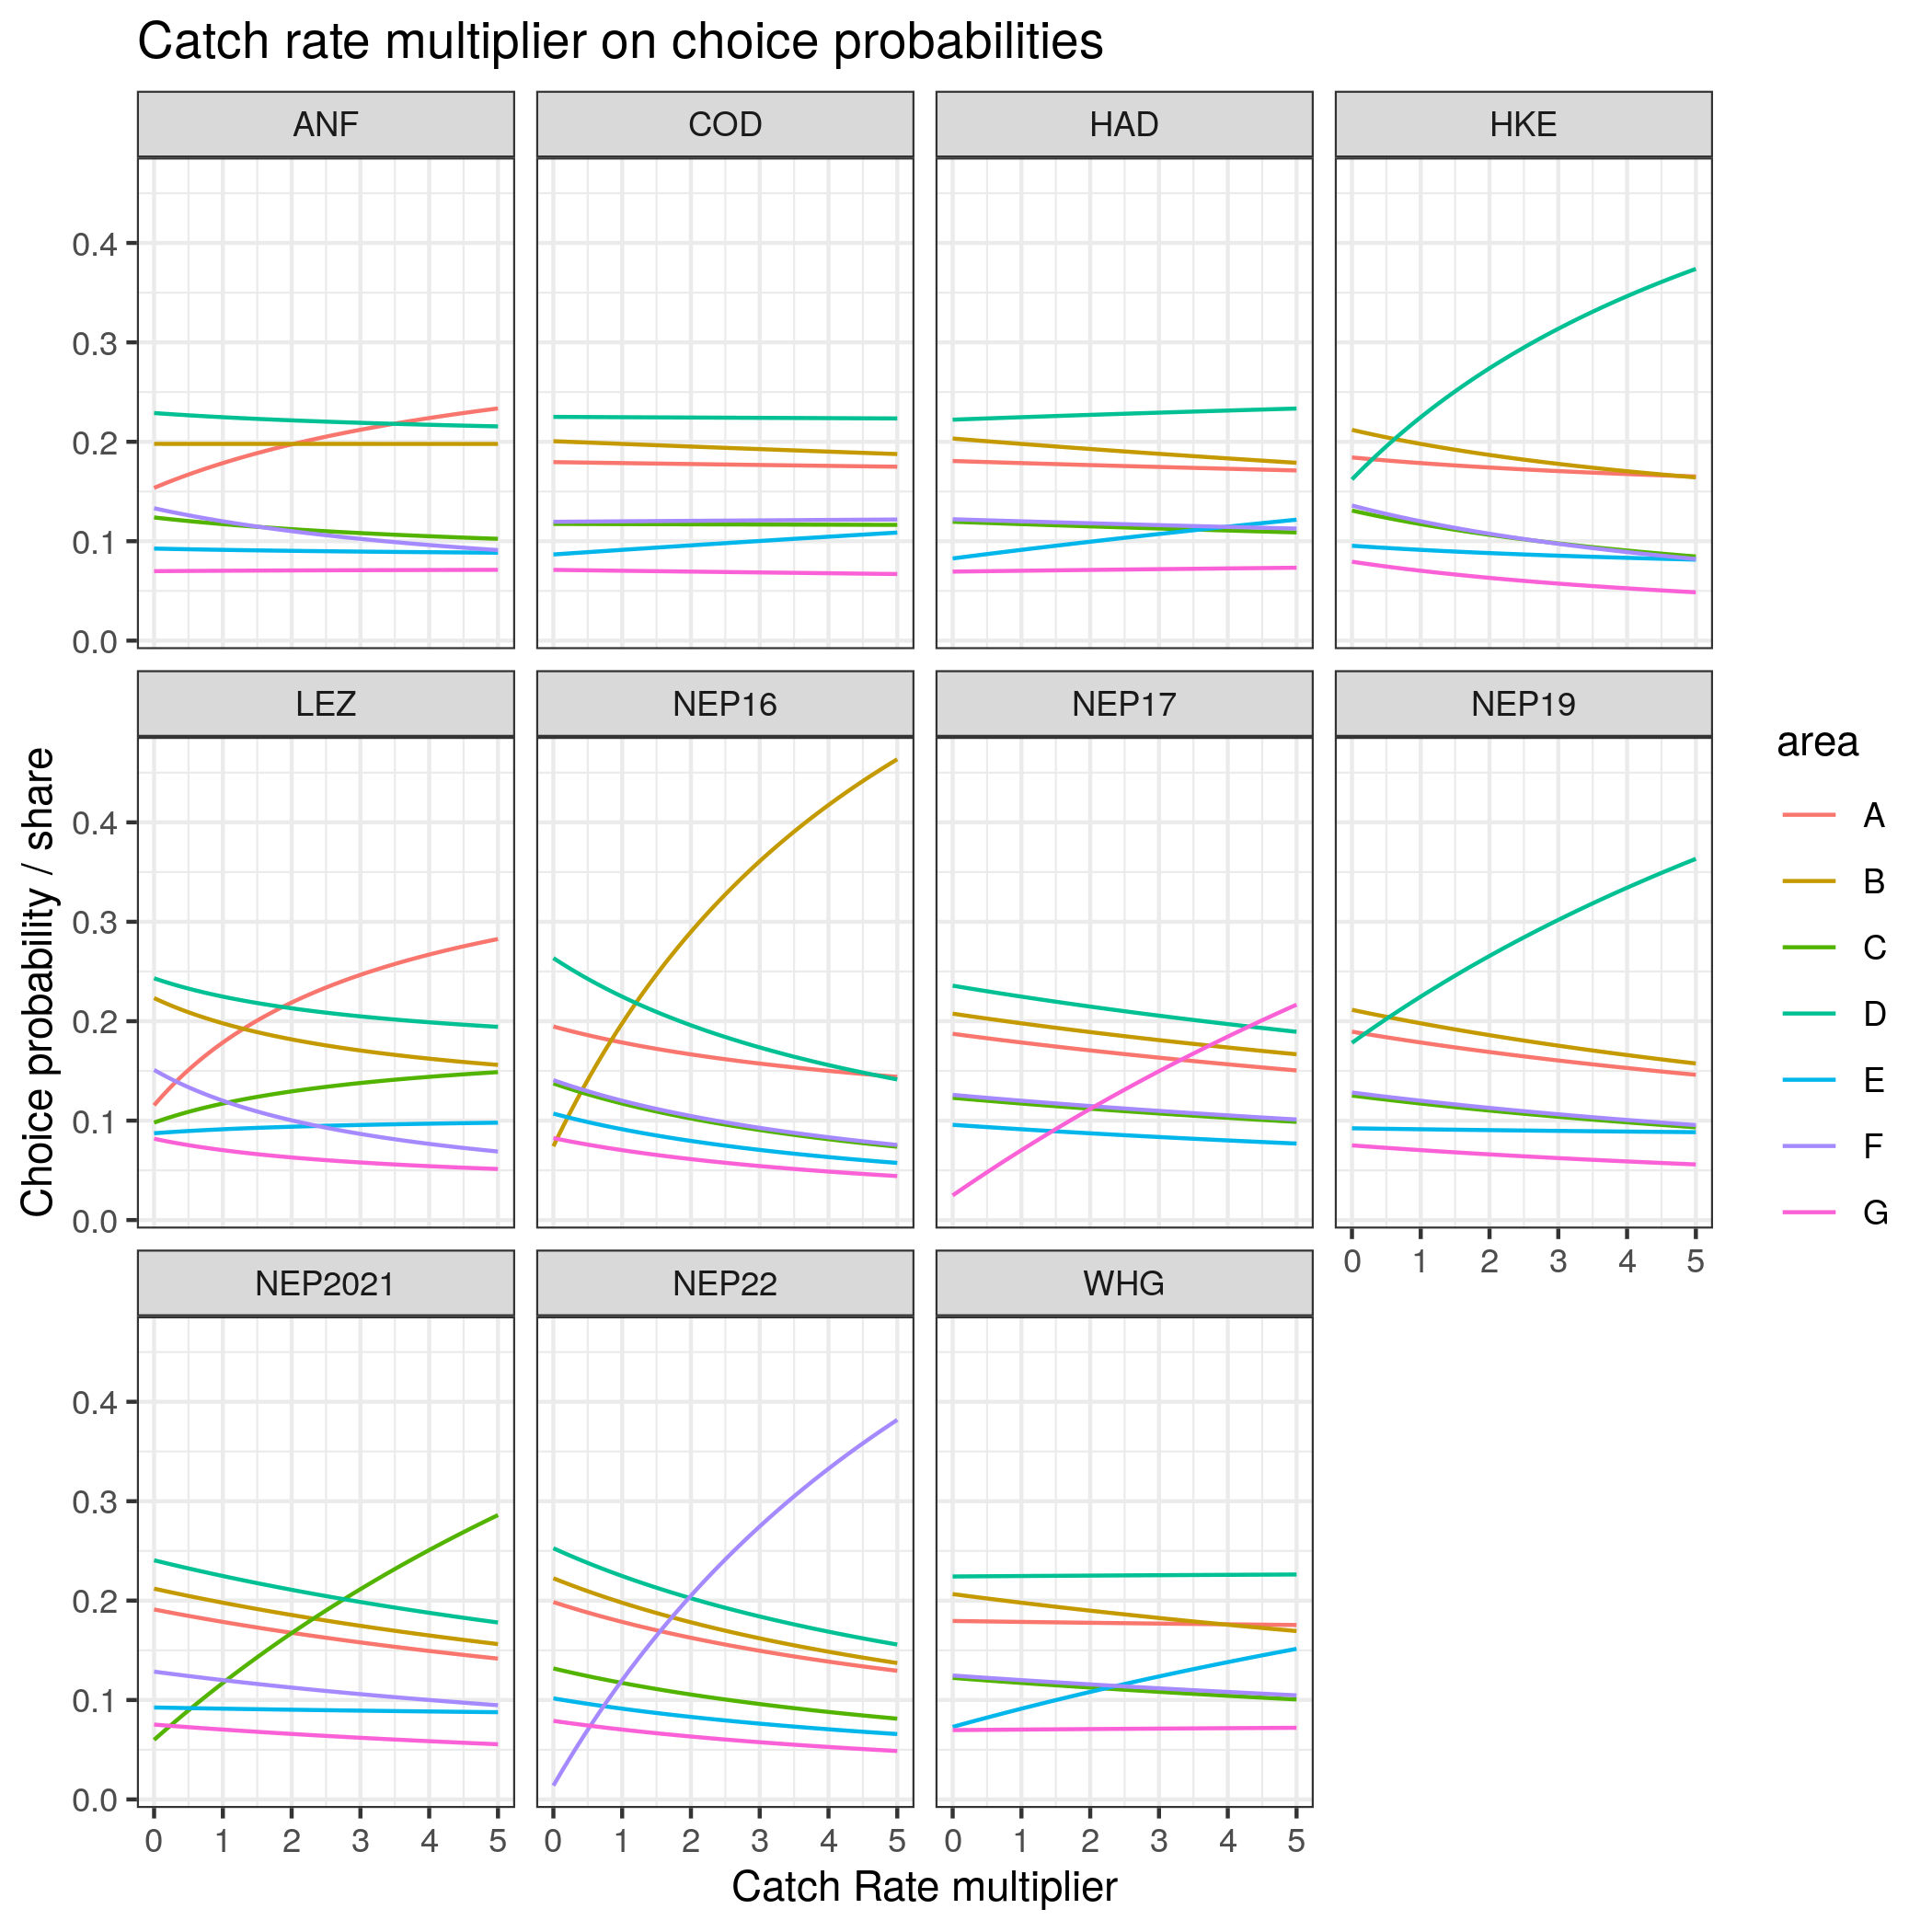
\includegraphics[width=1\linewidth]{figures/Gravity_Metier_Catch_Rate_Multiplier}
	\caption{The influence of changes in catch rates of different stocks on
	effort allocation among métier from the Gravity model.} 
	\label{fig:Grav_CR}
\end{figure}	

\begin{figure}[!ht]
	\centering
	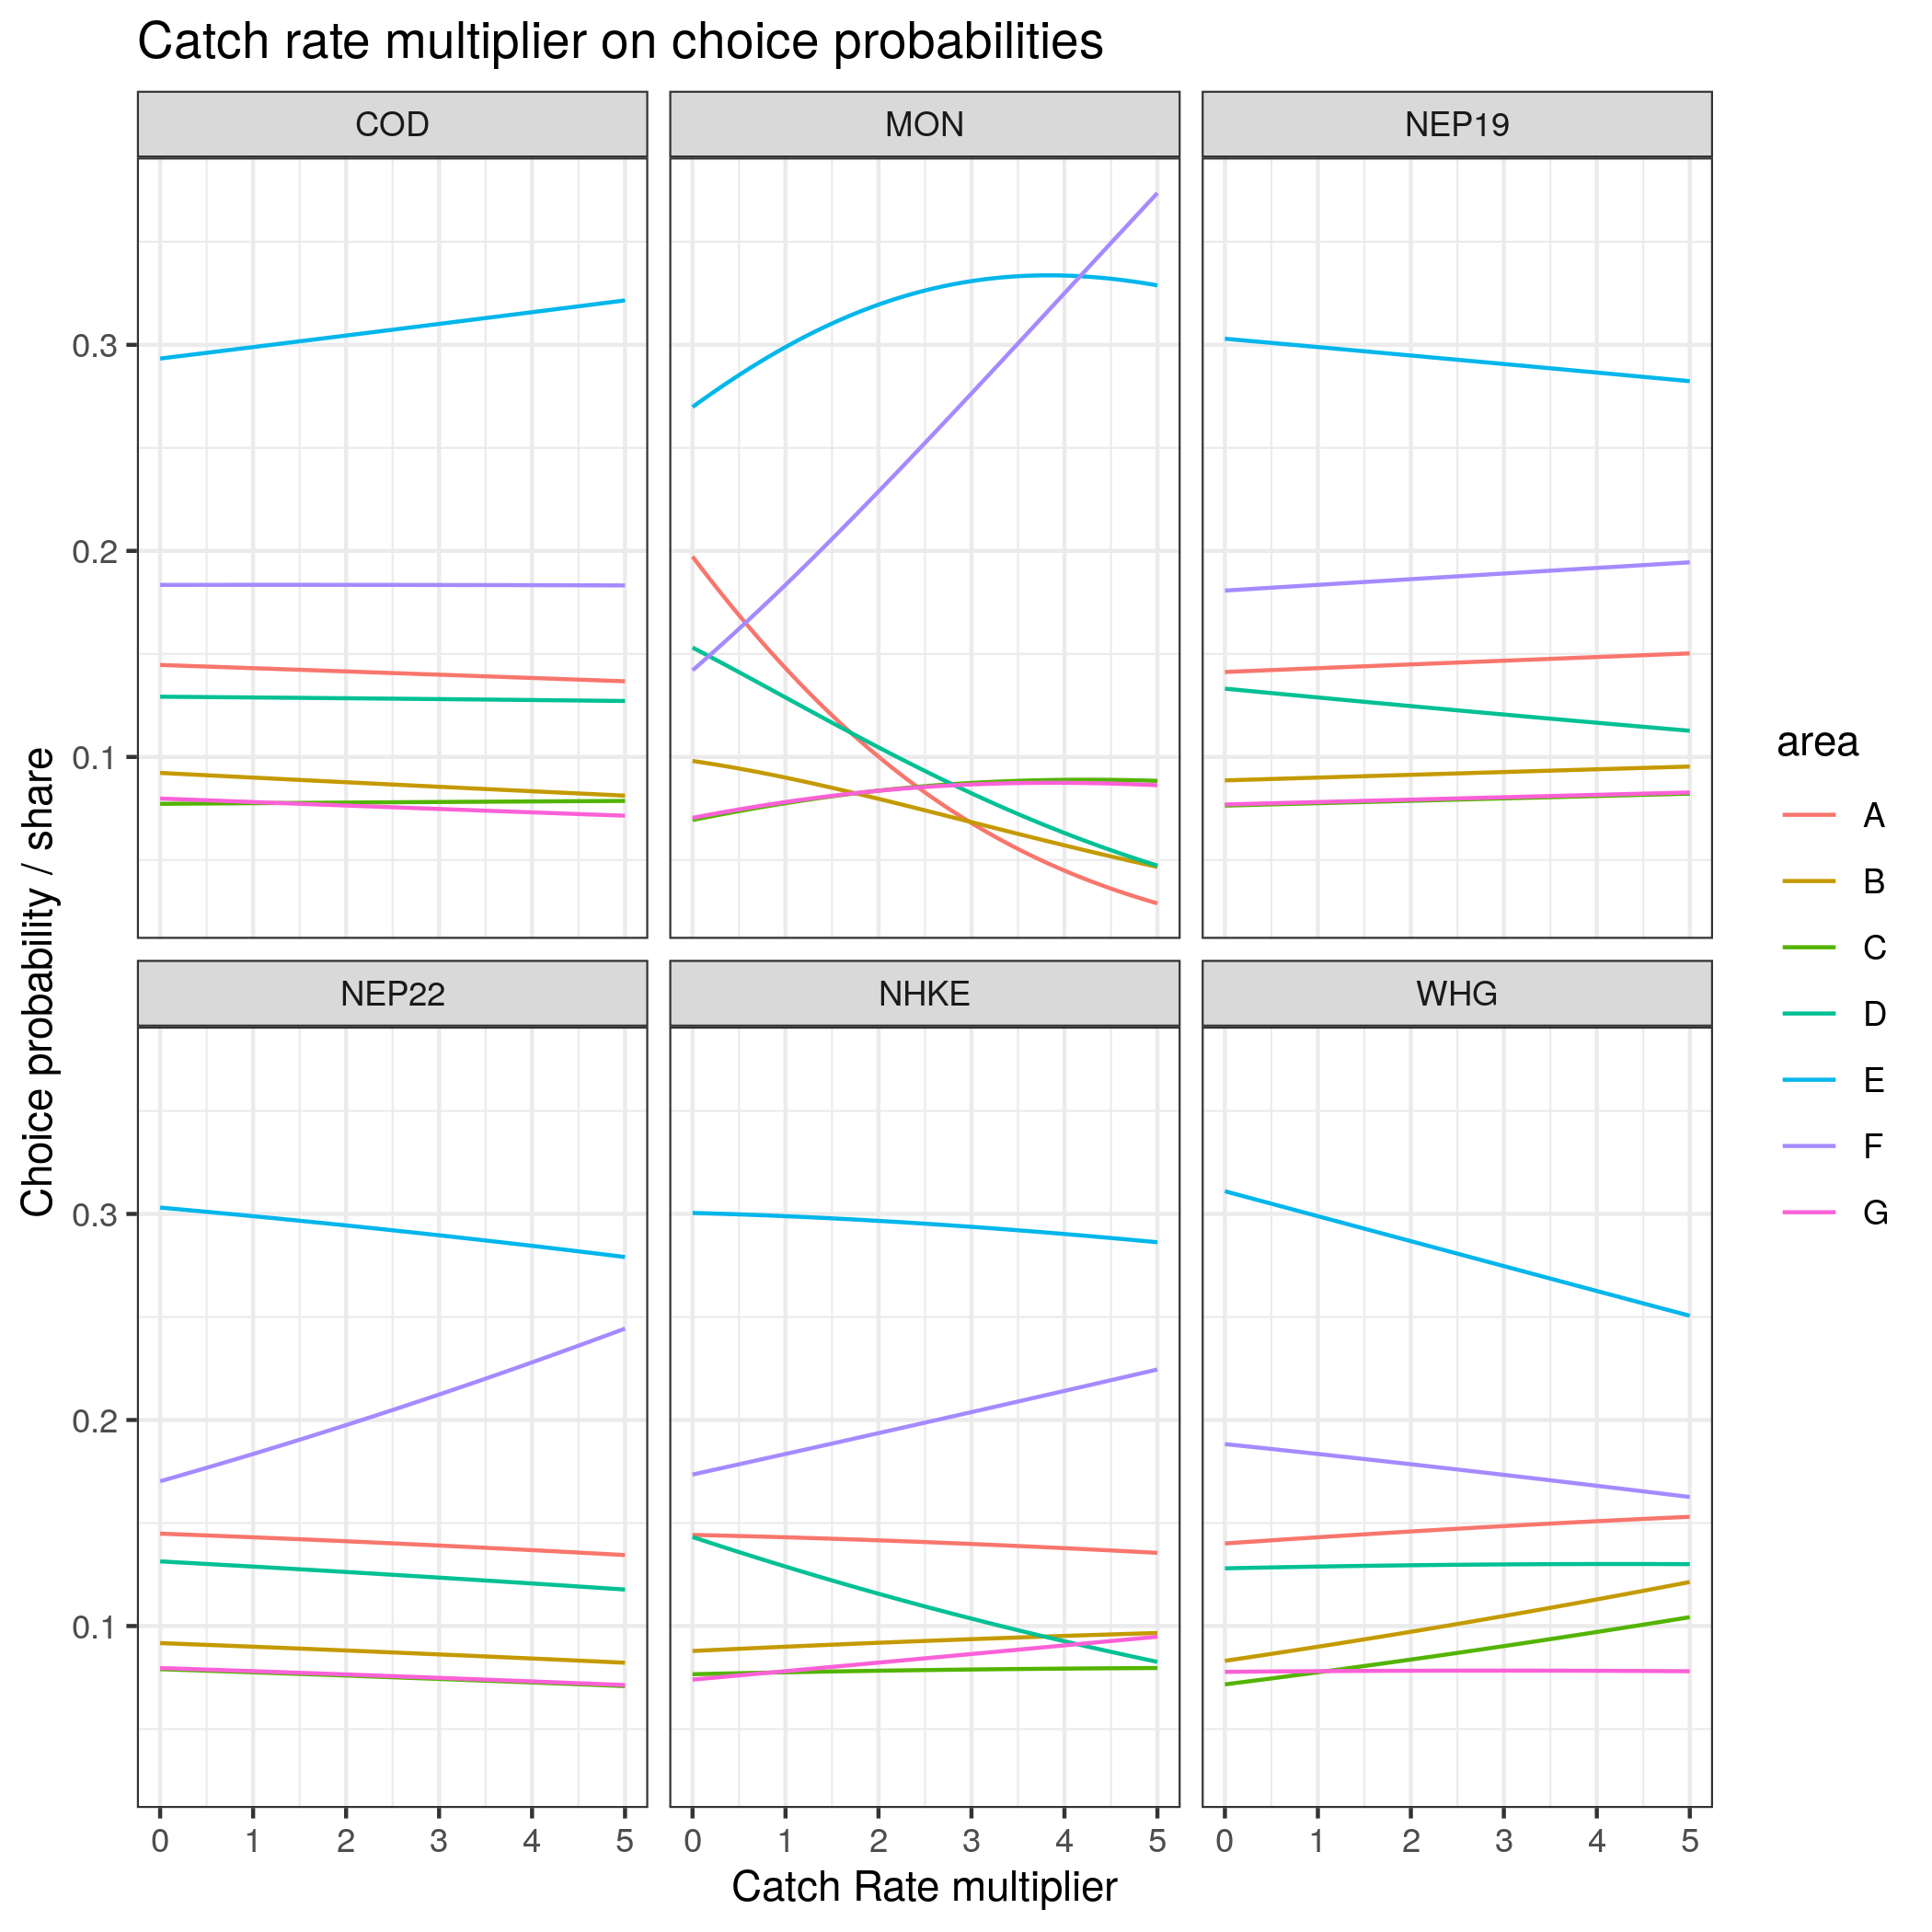
\includegraphics[width=1\linewidth]{figures/RUM_Metier_Catch_Rate_Multiplier}
	\caption{The influence of changes in catch rates of different stocks on
	effort allocation among métier from the RUM.} 
	\label{fig:RUM_CR}
\end{figure}	

\begin{figure}[!ht]
	\centering
	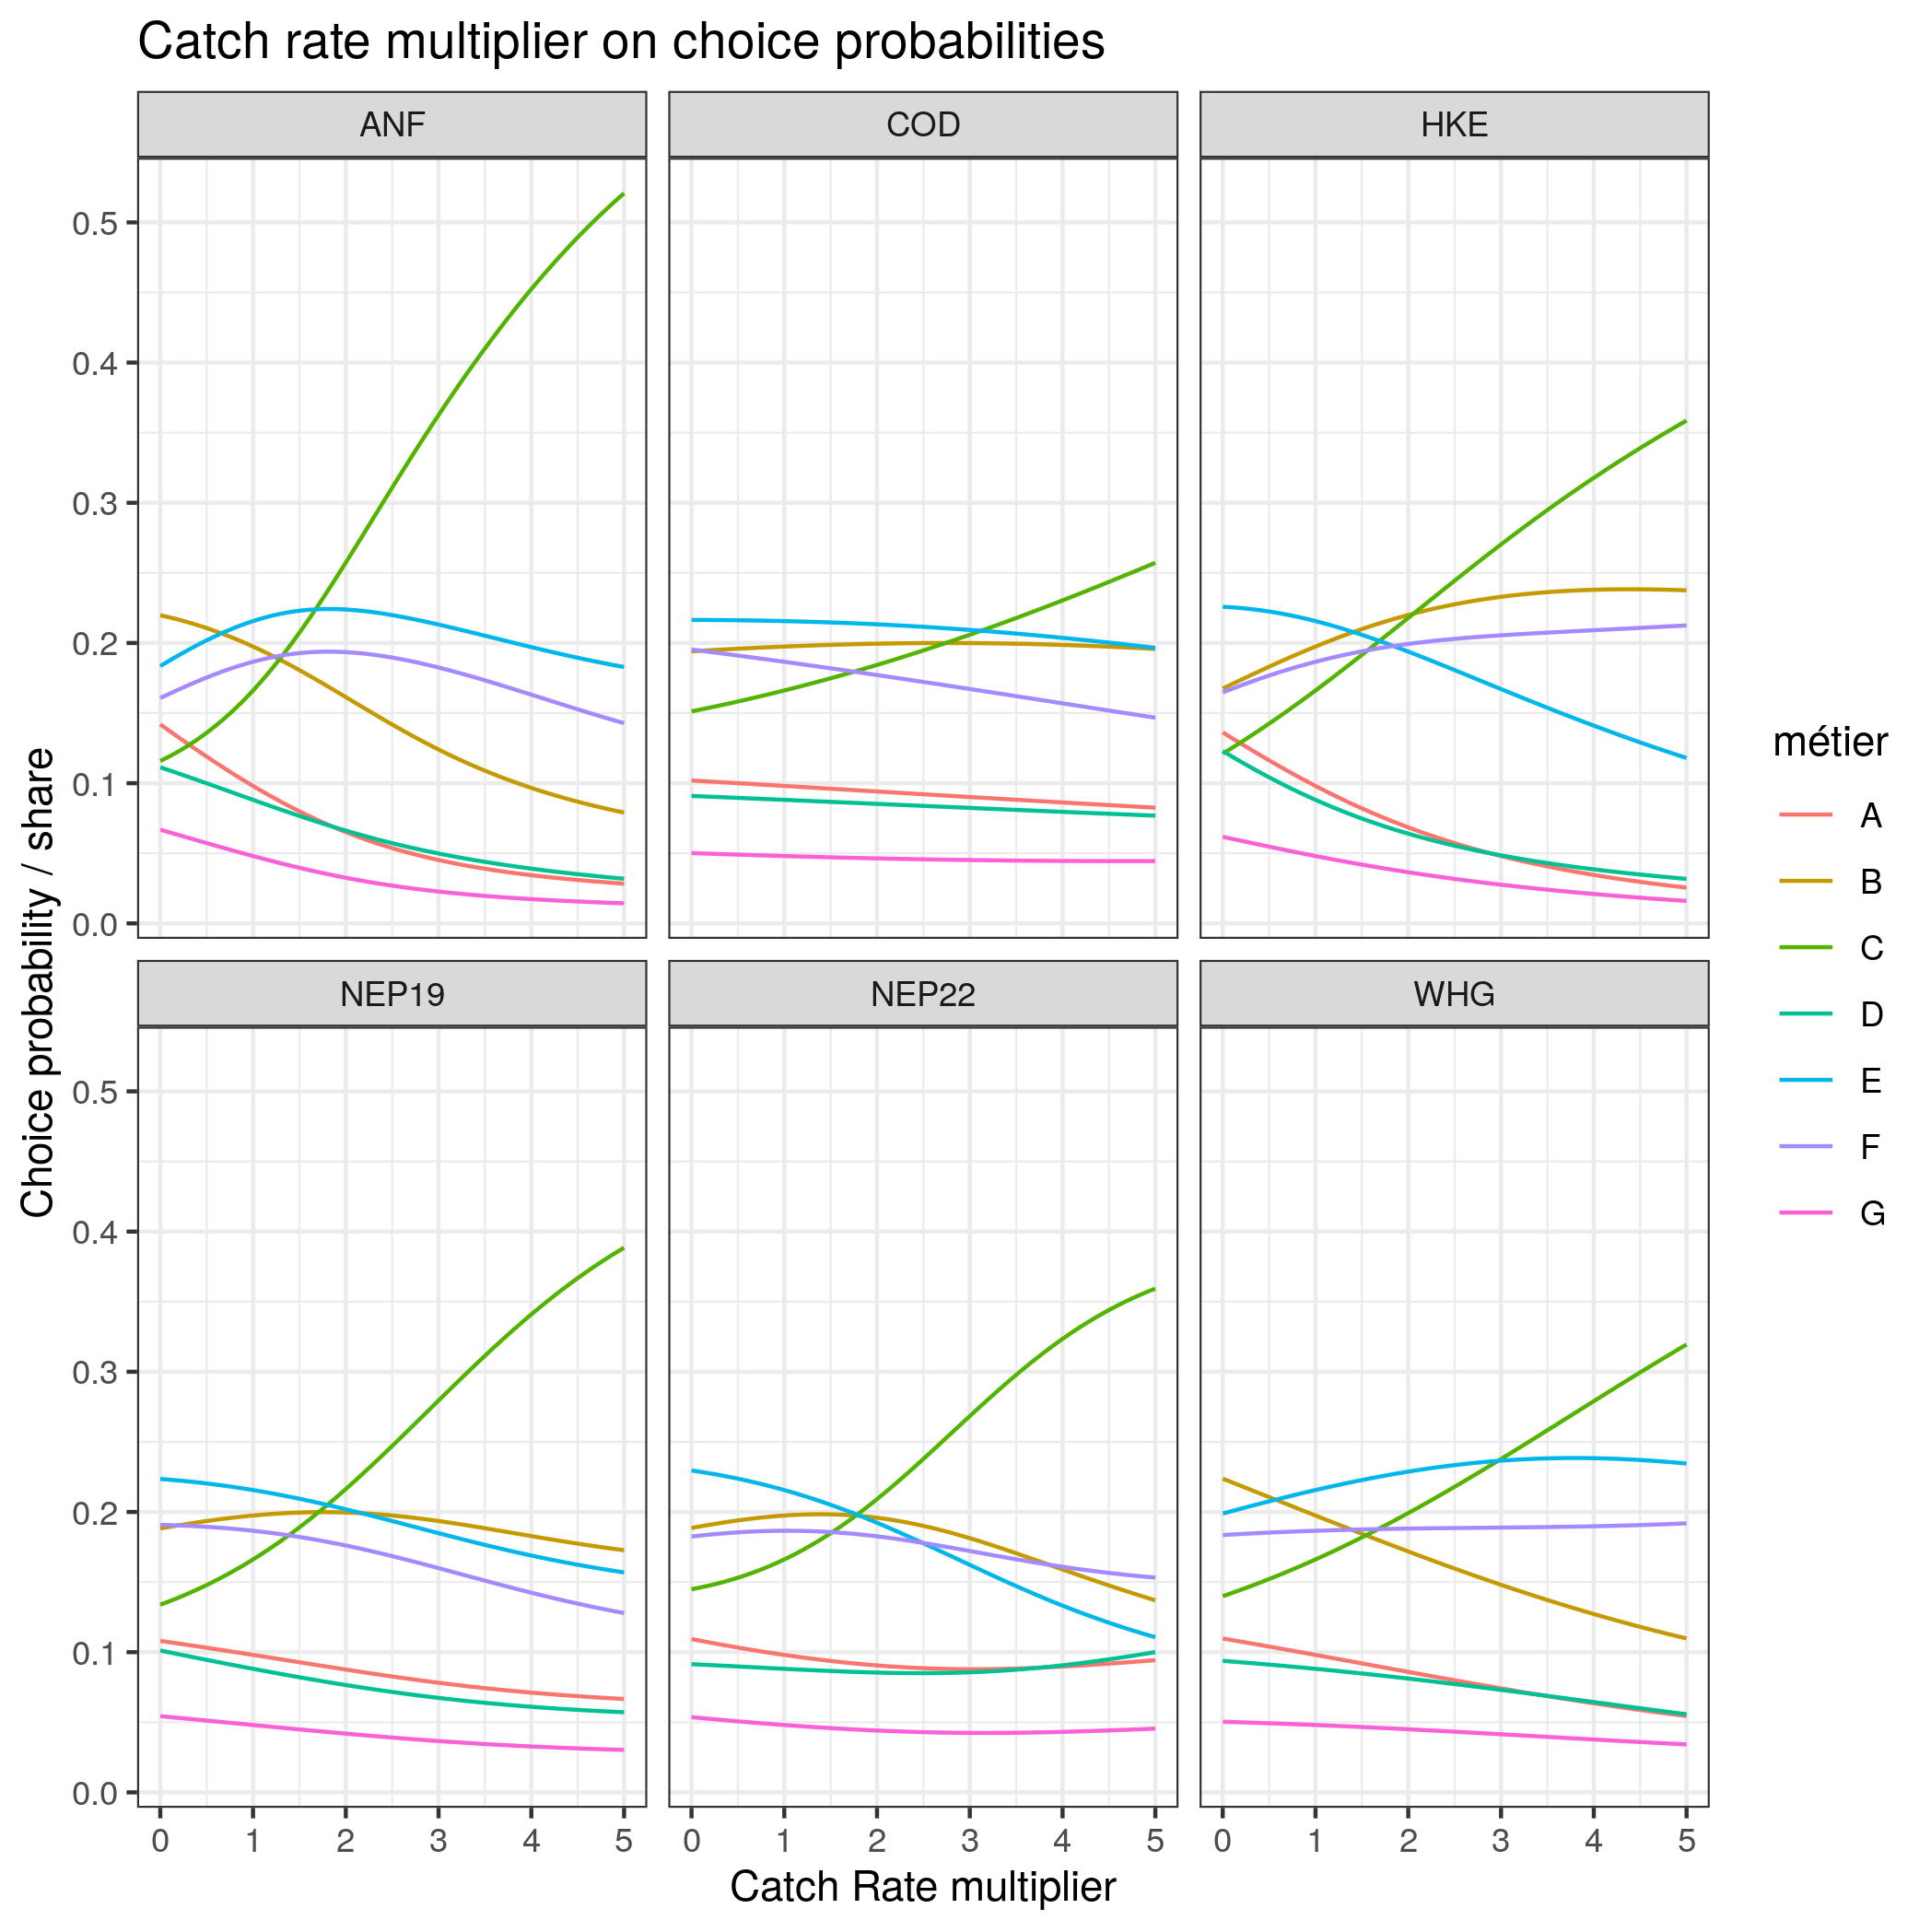
\includegraphics[width=1\linewidth]{figures/Markov_Metier_Catch_Rate_Multiplier}
	\caption{The influence of changes in catch rates of different stocks on
	effort allocation among métier from the Markov model.} 
	\label{fig:Markov_CR}
\end{figure}	

\begin{figure}[!ht]
	\centering
	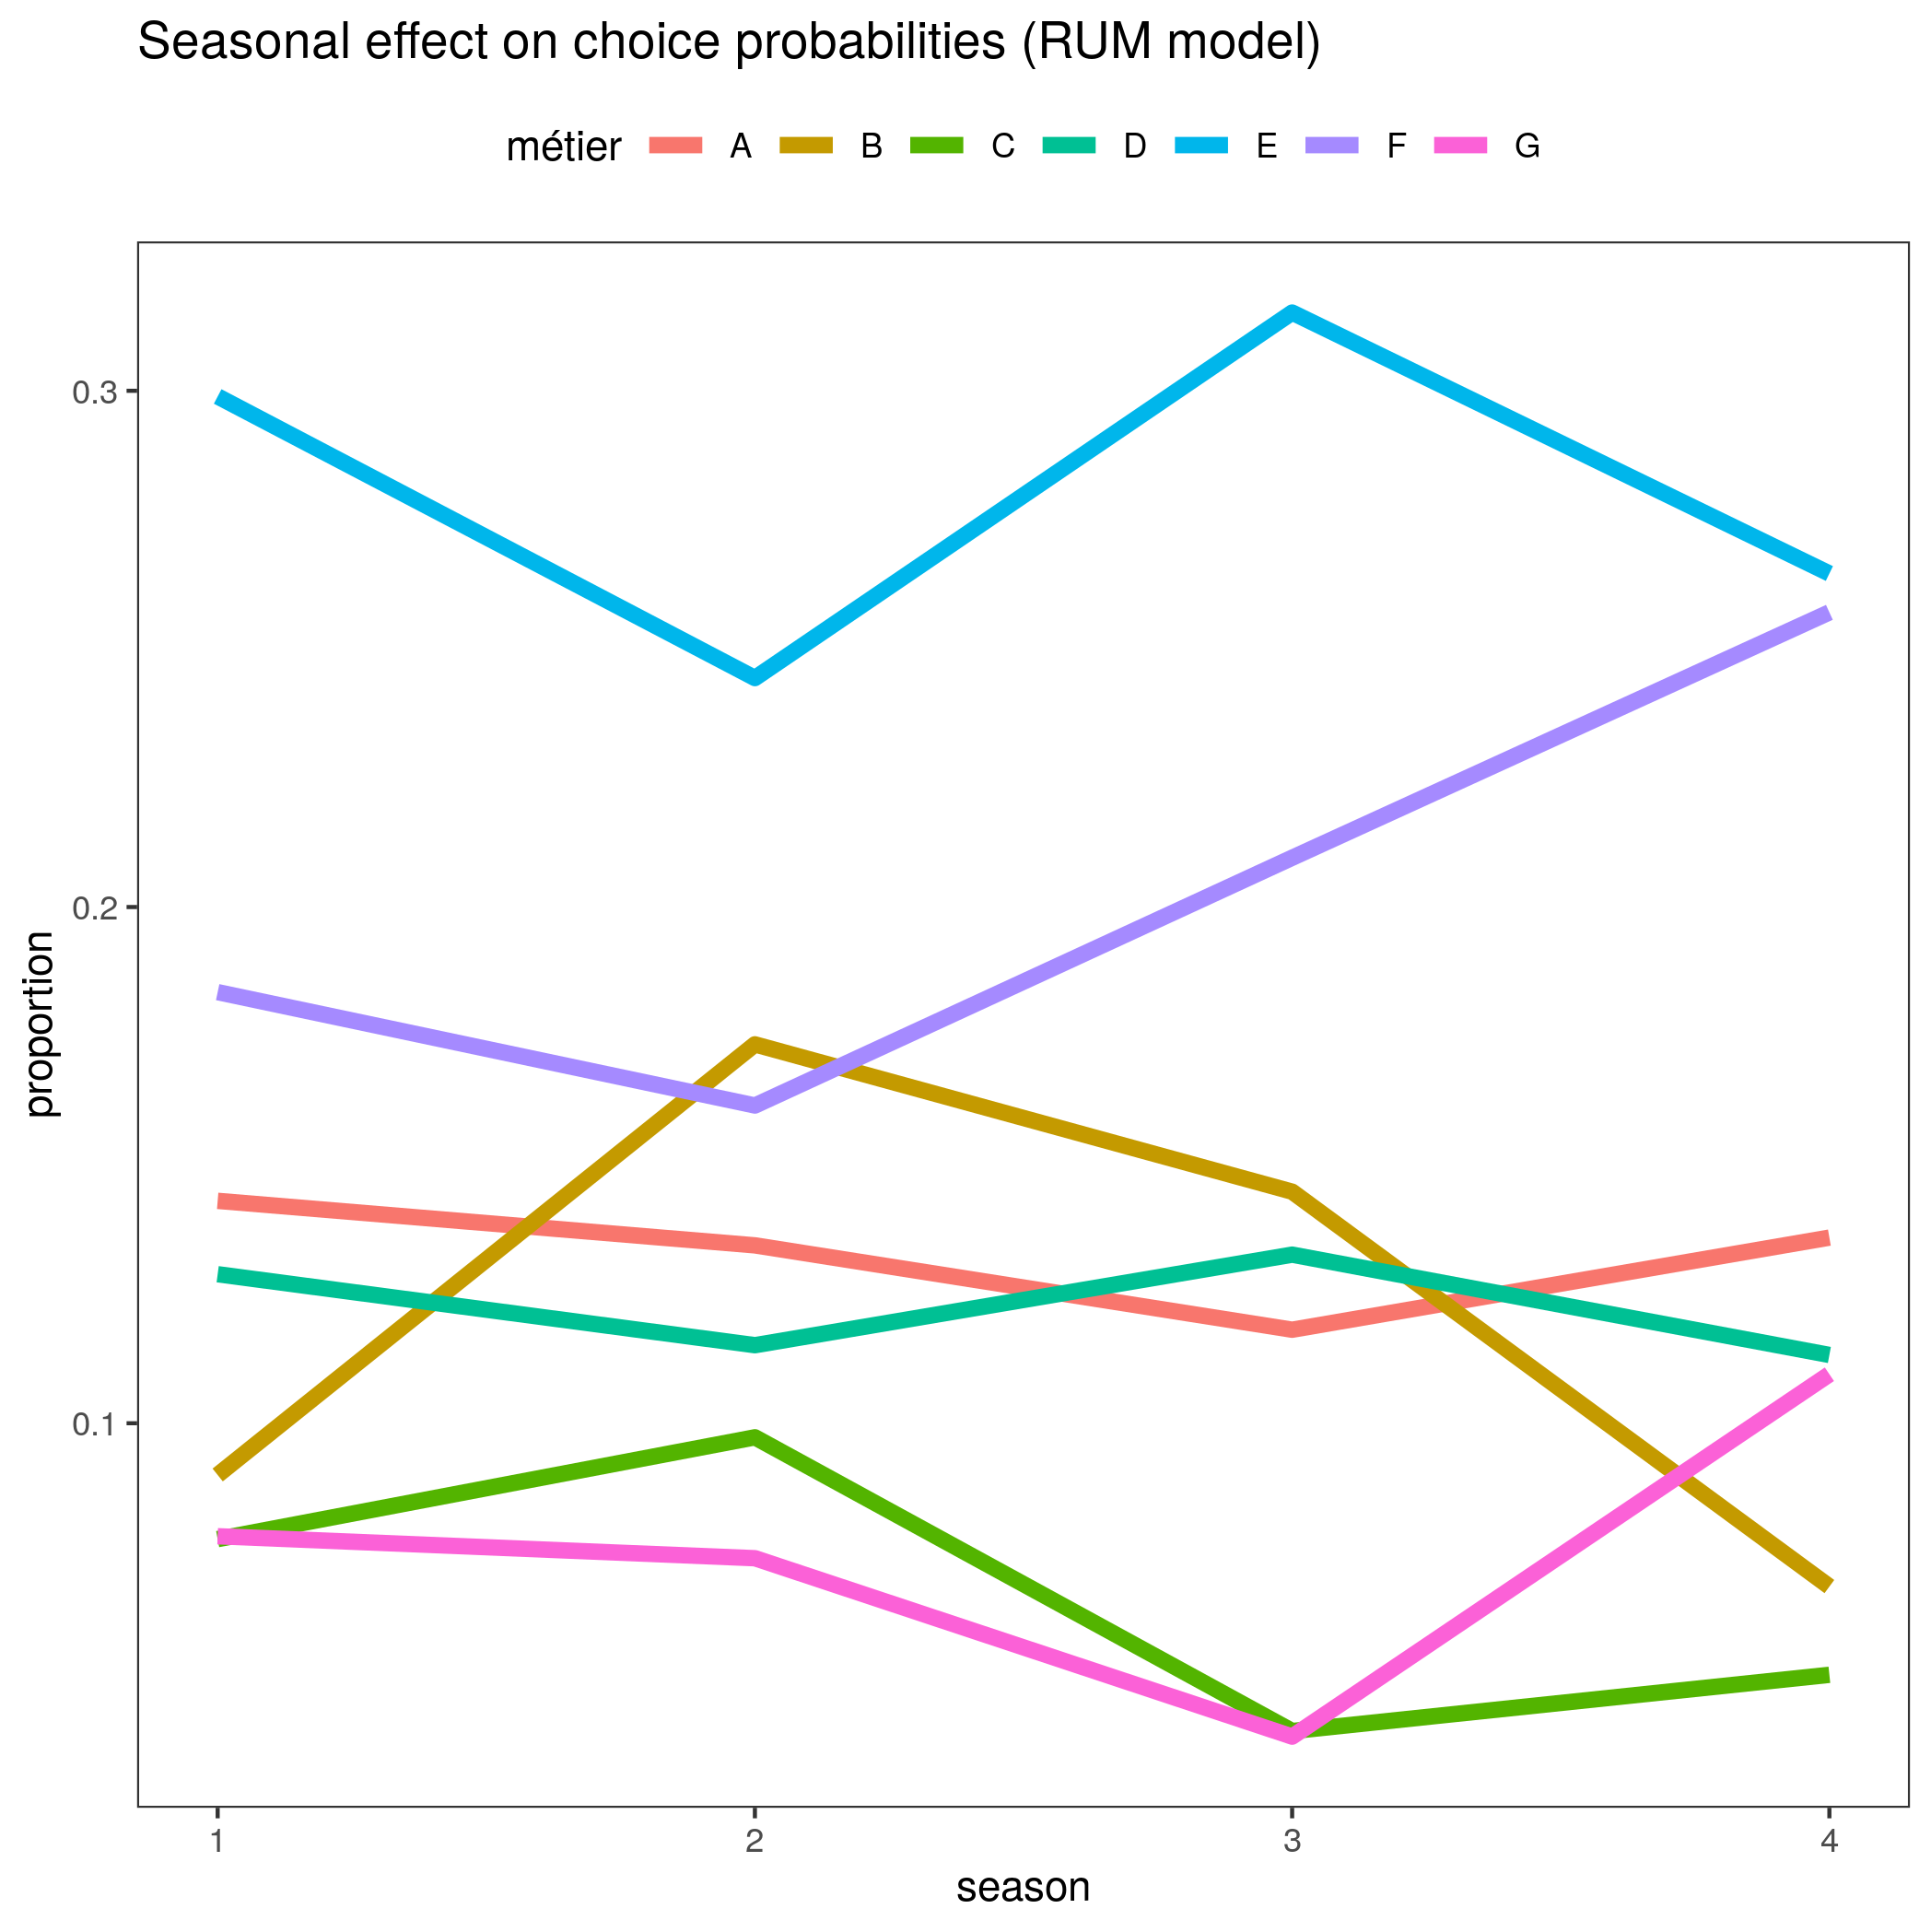
\includegraphics[width=1\linewidth]{figures/RUM_metier_seasonal_effect}
	\caption{Seasonal effect in the RUM model.} 
	\label{fig:RUM_Seas}
\end{figure}	

\begin{figure}[!ht]
	\centering
	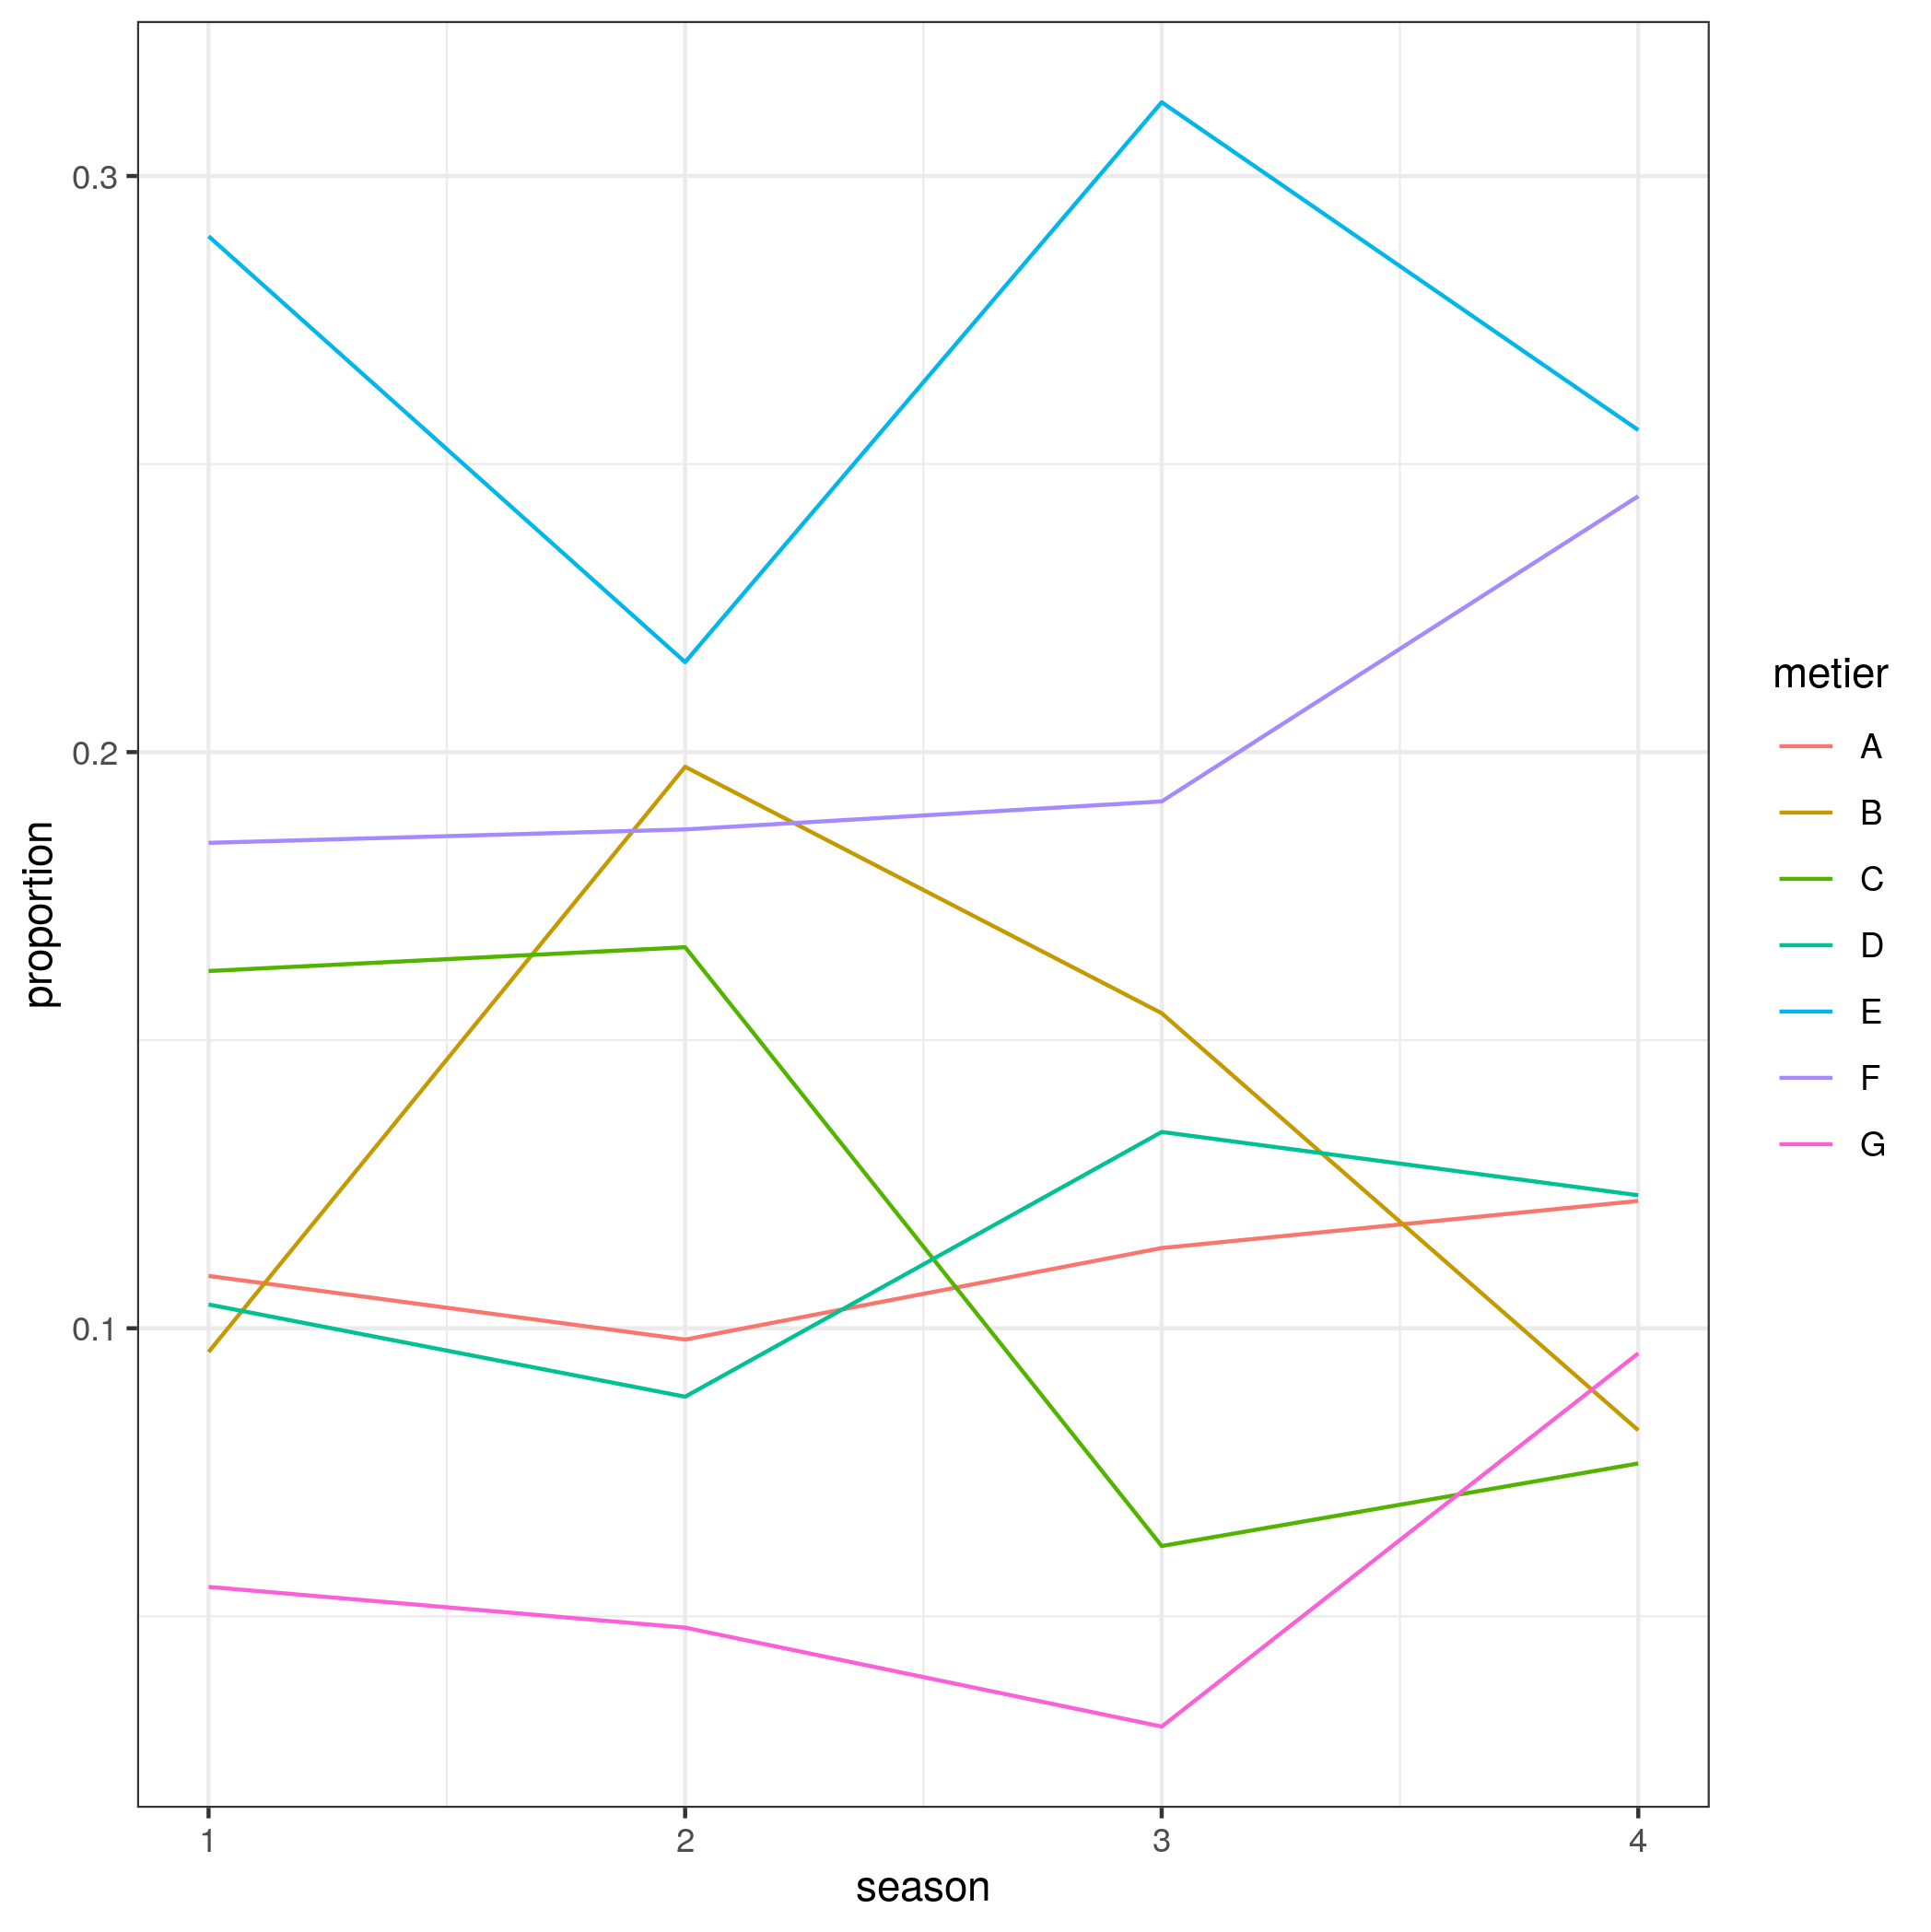
\includegraphics[width=1\linewidth]{figures/Markov_metier_seasonal_effect}
	\caption{Seasonal effect in the Markov model.} 
	\label{fig:Markov_Seas}
\end{figure}	




%%%%%%%%%%%%%%%%%%%%%%%%%
\end{document}
